\documentclass[oneside, 8pt]{amsart}
\usepackage{amscd, amsmath, amssymb, amsthm, amsfonts, amstext, verbatim, mathtools, xfrac, microtype, nameref, thmtools}
\usepackage[breaklinks=true,unicode]{hyperref}
\usepackage[hyperref=true, backend=biber, bibencoding=utf8, citestyle=numeric-comp, sortlocale=en_US, url=false, doi=false, eprint=true, maxbibnames=4]{biblatex}
\usepackage[capitalize]{cleveref}
\usepackage[matrix,arrow,curve]{xy}
\usepackage{tikz}
\usepackage{enumitem}
\usepackage[notref,notcite]{showkeys}

\addbibresource{paper.bib}
\renewbibmacro*{volume+number+eid}{\ifentrytype{article}{\- \iffieldundef{volume}{}{Vol.~\printfield{volume},}\iffieldundef{number}{}{ No.~\printfield{number},}}}
\renewbibmacro{in:}{\ifentrytype{article}{}{\printtext{\bibstring{in}\intitlepunct}}}
\newbibmacro{string+doi}[1]{\iffieldundef{doi}{\iffieldundef{url}{#1}{\href{\thefield{url}}{#1}}}{\href{http://dx.doi.org/\thefield{doi}}{#1}}}
\DeclareFieldFormat[article, inproceedings, inbook, book, thesis]{title}{\usebibmacro{string+doi}{\mkbibquote{#1}}}
\renewcommand*{\bibfont}{\footnotesize}

\newtheorem{prop}{Proposition}
\newtheorem{theorem}{Theorem}
\newtheorem{corollary}{Corollary}
\newtheorem{lemma}{Lemma}
\theoremstyle{remark} 

\theoremstyle{definition}
\newtheorem{df}[lemma]{Definition} \Crefname{df}{Definition}{Definitions}
\newtheorem{example}[lemma]{Example} \Crefname{example}{Example}{Examples}
\newtheorem{rem}[lemma]{Remark}
\newtheorem{cond}[lemma]{Condition}

\newlist{proplist}{enumerate}{1} \setlist[proplist]{label=(\roman{proplisti}), ref=\thethm.(\roman{proplisti}),noitemsep} \Crefname{proplisti}{Proposition}{Propositions}
\newlist{lemlist}{enumerate}{1} \setlist[lemlist]{label=(\roman{lemlisti}), ref=\thelem.(\roman{lemlisti}),noitemsep} \Crefname{lemlisti}{Lemma}{Lemmas}

\DeclareMathOperator{\Ker}{Ker}
\DeclareMathOperator{\Img}{Im}
\DeclareMathOperator{\St}{St}
\DeclareMathOperator{\GG}{G}
\DeclareMathOperator{\E}{E}
\DeclareMathOperator{\HH}{H}
\DeclareMathOperator{\K}{K}
\DeclareMathOperator{\GW}{GW}
\DeclareMathOperator{\colim}{colim}
\newcommand{\inv}{^{-1}}

\newcommand{\XX}{\mathcal{X}}           % (subset of) Steinberg generators
\newcommand{\RR}[1]{\mathcal{R}_{#1}}   % Steinberg relations
\newcommand{\catname}[1]{{\normalfont\textbf{#1}}} %Category name

\newcommand{\ZZ}{\mathbb{Z}}
\newcommand{\rA}{\mathsf{A}}
\newcommand{\rB}{\mathsf{B}}
\newcommand{\rC}{\mathsf{C}}
\newcommand{\rD}{\mathsf{D}}
\newcommand{\rE}{\mathsf{E}}
\newcommand{\rF}{\mathsf{F}}
\newcommand{\rG}{\mathsf{G}}

\numberwithin{equation}{section}

\title{On the presentation of orthogonal groups over polynomial rings}
\keywords {Steinberg group, $K_2$-functor, Serre problem
 {\em Mathematical Subject Classification (2010):} 19C20}
\author{Andrei Lavrenov}
\address{Mathematisches Institut der Universit\"at M\"unchen, Theresienstr. 39, D-80333 M\"unchen}
\email{avlavrenov at gmail.com}

\author {Sergey Sinchuk}
\address{Chebyshev laboratory, St. Petersburg State University, St. Petersburg, Russia}
\email {sinchukss at gmail.com}
\date {\today}

\begin{document}
\maketitle
\section{Introduction}


\section{Preliminaries}
$\langle \alpha, \beta \rangle = (\alpha, \beta^\vee) = (\alpha, \frac{2\beta}{(\beta, \beta)})$
Our convention for Cartan matrices is 
$A_{ij} = \langle \alpha_i, \alpha_j \rangle = (\alpha_i, \alpha_j^\vee)$.

\subsection{Steinberg groups}
%TODO: Describe what root systems are sympelctic and which are not
Let $\Phi$ be a reduced and irreducible root system of rank $\geq 2$ and $R$ be a commutative ring with $1$. Recall that in this case the \emph{Steinberg group} $\St(\Phi, R)$ can be defined by means of generators $x_{\alpha}(\xi)$ where $\xi\in R, \alpha\in\Phi$ and relations:
\begin{align}
& \phantom{[}
x_\alpha(s) x_\alpha(t) = x_\alpha(s+t),\ \alpha\in\Phi,\ s,t\in R; \label{rel:add}\\
& [x_\alpha(s), x_\beta(t)] = \prod\limits_{i,j\in\mathbb{N}}
 x_{i\alpha + j\beta}\left(N_{\alpha\beta ij}\, s^i t^j\right),\quad \alpha,\beta\in\Phi,\ \alpha\neq\pm\beta,\ s,t\in R. \label{rel:CCF}
\end{align}
The indices $i$, $j$ appearing in the right-hand side of the above relation range over
all positive natural numbers such that $i\alpha + j\beta\in\Phi$.
The structure constants $N_{\alpha \beta i j}=\pm 1,2,3$ appearing in \eqref{rel:CCF} depend only on $\Phi$ and can be computed explicitly.

Recall that for $\alpha\in\Phi$ and $s \in R^*$ the semisimple root elements $h_\alpha(s)$ are defined as follows: \[h_\alpha(s)=w_\alpha(s) \cdot w_\alpha(-1), \text{ where } w_\alpha(s) = x_\alpha(s) \cdot x_{-\alpha}(-s^{-1}) \cdot x_\alpha(s).\]

Recall from~\cite[Lemma~5.2]{Ma69} that the following identities hold for these elements:
 \begin{align} 
   \label{eq:conj-h-x} {}^{h_\alpha(t)}\!x_\beta(u) & = x_\beta(t^{\langle \beta,  \alpha \rangle}u) \\
   \label{eq:conj-h-h} {}^{h_\alpha(t)}\!h_\beta(u) & = h_\beta(t^{\langle \beta, \alpha \rangle} \cdot u) \cdot h_\beta(t^{\langle \beta,  \alpha \rangle})^{-1}.
 \end{align}

In our computations we will use two explicit elements of $\K_2(\Phi, R)$. Recall that Steinberg symbols are defined for any $s, t \in R^*$ by the identity
\begin{equation} \label{eq:steinberg} \{ s, t \}_\alpha = h_\alpha(s) \cdot h_\alpha(t) \cdot h_\alpha(st)^{-1}. \end{equation}

Recall also that Dennis--Stein symbols are defined for arbitrary $r, s\in R$ satisfying $1 + rs \in R^*$ as follows:
\begin{equation} \label{eq:dennis-stein}
 \langle r,s \rangle _ \alpha = x_{-\alpha}\left(\tfrac{- s}{1 + rs}\right) \cdot x_{\alpha}(r) \cdot x_{-\alpha}(s) \cdot x_{\alpha}\left(\tfrac{- r}{1+rs}\right) \cdot h_{\alpha}(1 + rs)^{-1}.
\end{equation} 
Notice that our notation follows~\cite{DS73} and {\it not}~III.5.11 of~\cite{Kbook}.

Dennis--Stein symbols and Steinberg symbols are related to each other via the following identities:
\begin{equation} \label{DS-S-relationship} \langle a, b \rangle_\alpha = \{-a, 1+ab\}_\alpha\text{ for } a, 1+ab\in R^*,\ \
 \{ s, t \}_\alpha = \left\langle -s, \tfrac{1 - t}{s} \right\rangle_\alpha\text{ for } s, t\in R^* \end{equation}

%Using~\eqref{eq:conj-h-h} it is easy to verify that \[[h_\alpha(s), h_\beta(t)] = \{s, t^{\langle \alpha, \beta \rangle}\}_\alpha = \{t, s^{\langle \beta, \alpha \rangle}\}_\beta^{-1}.\] 
It is easy to show that the above symbols depend only on the length of $\alpha$.
Moreover, if $\Phi$ is nonsymplectic, Steinberg symbols are antisymmetric and bimultiplicative, i.\,e. \begin{equation} \label{eq:symbol-properties} \{ u, st \} = \{ u, s\} \{ u, t \}, \ \{ u, v \} = \{ v, u\}^{-1}. \end{equation}

\begin{comment}
Suppose for a moment that $\langle \alpha, \beta \rangle = -1$ and  $\langle \beta, \alpha \rangle = -1$ then
\[ \{s, t^{-1} \} = \{s,  t^{-1}\}_\alpha = \{t, s^{-1} \}_\beta^{-1} = \{s^{-1}, t\} \]
In particular, $\{s, s^{-1}\} = \{s, s^{-1}\}^{-1}$ 
\end{comment}

\subsection{Unstable Quillen K-groups} \label{sec:quillen}
Throughout this section $G, P, S$ denote three group-valued functors on the category of commutative rings satisfying the following reqirements:
\begin{enumerate}
 \item \label{req:left-exact} $G$ is left exact;
 \item \label{req:subfunc} $P$ is a subfunctor of $G$ such that for all $R$ the group $P(R)$ is a perfect normal subgroup of $G(R)$;
 \item \label{req:uce} There is a natural transformation $\varphi \colon S \to P$ such that $ \varphi \colon S(R) \to P(R)$ is a universal central extension for all $R$;
 \item \label{req:coeq} $S$ preserves coequalizers of kernel pairs.
\end{enumerate}

Thanks to the functoriality of Quillen's plus-construction (see e.\,g.~\cite[Proposition~5.2.4]{Ro95}) one can define a functor 
%TODO: can also refer to Weibel's IV.1.5 provided Top is replaced with hTop which apparently does not change anything
$X_{G, P}(R) = BG(R)^+_{P(R)} \colon \catname{CRings} \to \catname{Top}$ and then define for $i \geq 1$ the corresponding K-group functors $\K_{i}(G, P, R)$ as the homotopy groups $\pi_i(X_{G, P}(R))$.

Let us also briefly recall Loday's procedure for relativization of $S$, that is,
 a way of extending $S$ from the category of rings to the category of pairs.
Denote by $p_0, p_1, \Delta$ the two obvious projections and the diagonal map $\xymatrix{D_{R,I} \ar@<1pt>[r] \ar@<-2.5pt>[r] & \ar@<-4pt>[l] R}$
  and set $d_i = Sp_i$, $s = S\Delta$.
 Obviously, $d_0s = d_1 s = id_{S(R)}$. Set $G_i = \Ker(d_i)$, and define $S(R, I)$ as $ G_0 / [G_0, G_1]$, denote by $\mu$ the natural map $S(R, I) \to S(R)$ induced by $d_1$.

%TODO: Give the definition of $D_{R, I}$ and of the category of Pairs
\begin{prop}\label{characterization}
\begin{enumerate}
 \item There are natural isomorphisms
  \[ \K_2(G, P, R) \cong \Ker(S(R) \to G(R)), \ \K_3(G, P, R) \cong \HH_3(S(R), \ZZ). \]
 \item The map $\mu \colon S(R, I) \to S(R)$ is the universal relative central extension of 
    the map $S(R) \to S(R/I)$. The kernel of $\mu$ is naturally isomorphic to the third relative homology group $\HH_3(S(R), S(R/I), \ZZ)$.
 \item There is a natural exact sequence:
 \[ \xymatrix{\K_3(G, P, R) \ar[r] & \K_3(G, P, R/I) \ar@{->>}[r] & \Ker(\mu).} \]
 \end{enumerate}   
\end{prop}
\begin{proof}
 The first claim follows from Exercises~1.8--1.9 of \cite[Chapter~IV]{Kbook} (here we use~\eqref{req:subfunc}--\eqref{req:uce}). %provided one verifies that all the intermediate isomorphisms are natural in $R$.
 
 Let us verify the second claim. From~\eqref{req:left-exact} and $\varphi(G_i) \subseteq \Ker(G(p_i))$ we conclude that $G_0 \cap G_1 \subseteq \Ker(\varphi \colon S(D_{R, I}) \to G(D_{R, I}))$
  therefore $G_0 \cap G_1$ is a central subgroup of $S(D_{R, I})$.
 From~\eqref{req:uce} we also obtain that $H_1(S(D_{R,I})) = H_2(S(D_{R,I})) = 0$ .
 The last two assertions allow us to invoke~\cite[Proposition~6]{Lo78} and conclude that the extension $S(R, I) \to S(R)$ is a universal relative central extension of the coequalizer $\mathrm{coeq}(d_0, d_1)$
  in the sense of~\cite[\S~3]{Lo78}. 
 Notice that this coequalizer coincides with $S(R) \to S(R/I)$ by~\eqref{req:coeq}. 
 Finally, the kernel of $\mu$ is isomorphic to $\HH_3(S(R), S(R/I), \ZZ)$ by~\cite[Th{\'e}or{\`e}me~2]{Lo78}.
 
 The third claim now follows from the starting portion of the homology long exact sequence of the map $S(R) \to S(R/I)$ and the first two assertions.
\end{proof}

Let us mention the example of a triple $(G,P,S)$ satisfying the above conditions.
\begin{example} \label{ex:orth}
 For $n \geq 5$ take the orthogonal group functor $\mathrm{O}_{2n}(-)$ and its elementary subfunctor $\mathrm{EO}_{2n}(-)$ as functors $G_n$ and $P_n$, respectively.
 Now set $S_n = \St(\rD_n, -)$.
 From [Stein's paper] and [Lemma on centrality] it follows that $S_n$ and $P_n$ satisfy~\eqref{req:uce}.
 The other requirements can be verified in a straightforward manner.
\end{example}

In the above definition we could have replaced the group $\mathrm{O}_{2n}$ with a different isogeneous form of the orthogonal group, e.\,g. 
 we could have chosen $G_n = \mathrm{SO}_{2n}$ or $G_n = \mathrm{Spin}_{2n}$ and then have defined $P_n$ as its elementary subfunctor.
Of course, this would change the functors $\K_i(G_n, P_n, -)$ for $i=1,2$ however, as the proof of~\cref{characterization} suggests %TODO: Does it really change K_2?
 it would not change $\K_i(G_n, P_n, -)$ for $i\geq 3$.

Now let $G_n, P_n$ be again as in~\cref{ex:orth}. We write $KO_i(n, R)$ as a shorthand for $\K_i(G_n, P_n, R)$.
Let us formulate the stability theorem for orthogonal Quillen K-groups (see~\cite[Theorem~9.4]{Pa89}).
\begin{theorem}[Panin] \label{lem:Panin-stability}
 Let $R$ be either a field, principal ideal domain or a Dedekind domain. Set $a = 1,2$ or $3$ in each of these respective cases.
 Then the canonical map $KO_i(2n, R) \to KO_i(2(n+1), R)$ is an epimorphism for $n \geq b$ 
 and an isomorphism for $\ell \geq b + 1$, where $b = \mathrm{max}(2i, a+i-1)$. \end{theorem}
 
Of course, the limit groups $\K_i(\mathrm{O}_\infty, \mathrm{EO}_\infty, R) = KO_i(R)$ are exactly hermitian K-groups ${}_{-1}\!L_i(R)$ defined in~\cite{Ka80}.
There is a modern version of hermitian K-theory, namely the theory of higher Grothendieck--Witt groups of schemes.
We refer the reader to~\cite[\S~2]{AF17} or~\cite[\S~2]{FRS12} for an introduction to this theory.
For our purposes it would be sufficient to restrict our attention to to the affine case and to think of $\GW_i^{[k]}(R)$ as a shorthand for
\begin{equation}
 \GW_i^{[k]}(R) = \left\{\begin{array}{ll} KO_i(R), & k = 0, \\ U_i(R), & k = 1, \\ KSp_i(R), & k = 2, \\ {}_{-1}\!U_i(R), & k = 3. \end{array}\right.
\end{equation} %TODO: Reference?
The groups ${}_{\pm 1}\!U_i(R)$ are defined in~\cite{Ka80} and we will not use their definition.
The notation for the upper index $[k]$ suggests that Grothendieck--Witt groups are $4$-periodic in $k$.


In the sequel we will need the following result.
\begin{theorem}[Bass Fundamental Theorem]\label{bass-ft} Suppose that $2 \in R^*$, then for any $i\geq 1$, $k\in \ZZ/4\ZZ$ there is a natural split exact sequence of abelian groups
 \[ \xymatrix{ 0 \ar[r] & \GW_i^{[k]}(R) \ar[r] & \GW_i^{[k]}(R[X, X^{-1}]) \ar[r]  & \GW_{i-1}^{[k-1]}(R) \ar[r] & 0.} \] \end{theorem}
\begin{proof} This is a special case of~\cite[Theorem~9.13]{Sch16} and the remark that follows it. \end{proof}

\subsection{Relative Steinberg groups}
Let us briefly recall the definition and basic properties of relative Steinberg groups.
We refer the reader to~\cite[Section~3]{S15} for a more detailed exposition.
By definition, the relative Steinberg group functor $\St(\Phi, R, I)$ is obtained from the functor $\St(\Phi, R)$
 via the relativization procedure described in~\cref{sec:quillen}.

\begin{lemma}\label{lem:lemma32} Let $\Phi$ be a simply-laced root system of rank $\geq 3$,
$A$ be arbitrary commutative local ring with maximal ideal $M$ and residue field $k$.
Denote by $B = B_{A, M}$ the subring $A[X^{-1}] + M[X]$ of the ring $R = A[X, X^{-1}]$ and
by $I$ the ideal $M[X, X^{-1}]$ of $B$ (it is clear that $I$ is also an ideal of $R$).
Consider the following commutative square of canonical maps.
\[ \xymatrix{
    \St(\Phi, B, I) \ar[r] \ar[d] & \St(\Phi, B) \ar[d] \\
    \St(\Phi, R, I) \ar[r] \ar@{-->}[ur] & \St(\Phi, R) } \]
Then there exists a diagonal arrow which makes the diagram commute.   
\end{lemma} 
\begin{proof}
 Notice that $R$ is isomorphic to the principal localisation of $B$ at $X$
  and that $I$ is uniquely $X$-divisible in the sense of~\cite[\S~4]{LS17}.
 Thus, in the special case $\Phi = \rA_3$ the assertion of the lemma follows from~\cite[Theorem~3]{LS17}.
 
 Now the general case can be obtained as a corollary of amalgamation theorem~\cite[Theorem~9]{S15}
  (cf.~\cite[\S~4]{LS17} for more details).
\end{proof}
%TODO: Give reference on a similar result of Lavrenov?

If we denote the kernel of the natural transformation $\mu$ from the definition of $\St(\Phi, R, I)$ by $C(\Phi, R, I)$ we obtain a natural exact sequence:
\begin{equation} \label{relSteinberg-def}
 \xymatrix{ 1 \ar[r] & C(\Phi, R, I) \ar[r]^{j} & \St(\Phi, R, I) \ar[r]^{\mu} & \St(\Phi, R) \ar[r]^{\pi} & \St(\Phi, R/I) \ar[r] & 1.}
\end{equation}
The group $C(\Phi, R, I)$ is trivial when $I$ is a splitting ideal of $R$, i.\,e. when the canonical map $R \to R/I$ splits.
This immediately follows e.\,g. from the exact sequence of~\cref{characterization}, it is also possible to give a direct proof of this fact, see \cite[Lemma~8]{S15}.
The following result plays a key role in the proof of~\cref{thm41}.
\begin{lemma} \label{lem:prop41}
In the notation of~\cref{lem:lemma32} assume additionally that the residue field $k$ is of characteristic $\neq 2$.
Then the canonical map $f\colon C(\rD_\ell, B, I) \to C(\rD_\ell, R, I)$ is surjective for $\ell \geq 7$.
\end{lemma}
\begin{proof}
  Consider the following commutative diagram with rows obtained from~\cref{characterization}:
\begin{equation*}\xymatrix{
 KO_3(2\ell, B) \ar[r] \ar[d] & KO_3(2\ell, k[X]) \ar[d]_{f'} \ar@{->>}[r] & \ar[d]_{f} C(\rD_\ell, B, I) \\
 KO_3(2\ell, R) \ar[r]        & KO_3(2\ell, k[X, X^{-1}]) \ar@{->>}[r]        & C(\rD_\ell, R, I).}\end{equation*}
In view of~\cref{lem:Panin-stability} the central vertical map $f'$ is isomorphic to the canonical map $\GW_3^{[0]}(k[X]) \to \GW_3^{[0]}(k[X, X^{-1}])$.
Invoking~\cref{bass-ft} we obtain that \[\GW_3^{[0]}(k[X, X^{-1}]) \cong \GW_3^{[0]}(k) \oplus \GW_2^{[3]}(k).\]
By \cite[Lemma~2.2]{FRS12} the group $\GW_2^{[3]}(k)$ is trivial, therefore $f'$ (and hence $f$) are surjective.
\end{proof}

\subsection{Some elementary lemmas}
\begin{comment}
Hall-Witt identity
\[ [[ y^{-1}, x], z] ^ {y^{-1}}  [[ z^{-1}, y], x] ^ {z^{-1}}  [[ x^{-1}, z], y] ^ {x^{-1}} = 1 \]
\[ [[ y^{-1}, x], z]  \cdot [[ z^{-1}, y], x] ^ {z^{-1}y} \cdot  [[ x^{-1}, z], y] ^ {x^{-1}y} = 1. \]
\[ [[ z^{-1}, y^{-1}], x] ^ {z^{-1}y^{-1}} \cdot  [[ x^{-1}, z], y^{-1}] ^ {x^{-1}y^{-1}} = [z, [ y, x]] . \]
\[  . \]
\end{comment}
Throughtout this section $A$ denotes an arbitary ring and $I, J$ two its ideals and $\Phi$ a simply laced root system.

The following lemma summarizes basic properties of structure constants which will be used in the computations below, often without explicit reference.
\begin{lemma} Suppose $\alpha, \beta \in \Phi$ are such that $\alpha+\beta \in \Phi$.
\begin{enumerate}\label{lem:structure-constants}
 \item $N_{\alpha, \beta} = -N_{\beta,\alpha}$;
 \item $N_{\alpha, \beta} = - N_{-\alpha, -\beta}$;
 \item $N_{\alpha, \beta} = N_{\beta, -\alpha-\beta} = N_{-\alpha-\beta, \alpha}.$
\end{enumerate}
\end{lemma}
\begin{proof} See~\cite[\S~14]{VP}. \end{proof}

We define the following two families of elements of $\St(\Phi, A)$:
\begin{itemize}
 \item $z_\alpha(s, \xi) := x_\alpha(s)^{x_{-\alpha}(\xi)}$ defined for $\xi \in A$, $s \in I$;
 \item $c_\alpha(s, t) = [x_\alpha(s), x_{-\alpha}(t)]$ defined for $s \in I$, $t \in J$.
\end{itemize}

\begin{lemma}\label{Zrels} The elements $z_\alpha(s, \xi)$ satisfy the following relations for all $\xi, \eta\in A$, $s\in I$:
\begin{enumerate} 
\item\label{Z1} $z_{\alpha}(s, \xi) ^ {x_{-\alpha}(\eta)} = z_{\alpha}(s, \xi + \eta)$;
\item\label{Z2} $z_{\beta}(s, \xi) ^ {x_{\alpha}(\eta)} = x_{\alpha} (- s\xi \eta) \cdot x_{\alpha+\beta} (N_{\beta, \alpha}\cdot s\eta)     \cdot z_{\beta}(s, \xi)\ \text{if}\ \alpha + \beta \in \Phi$;
\item\label{Z3} $z_{\beta}(s, \xi) ^ {x_{\alpha}(\eta)} = x_{\alpha} (s\xi \eta) \cdot x_{\alpha-\beta} (N_{\beta,-\alpha}\cdot s\xi^2\eta) \cdot z_{\beta}(s, \xi)\ \text{if}\ \alpha - \beta \in \Phi$;

\item\label{Z4} $z_{\beta}(s, \xi) ^ {x_{\alpha}(\eta)} = z_{\beta}(s, \xi)\ \text{if}\ \alpha\perp\beta$;
\item\label{Z5} If $\alpha+\beta\in\Phi$, then holds:
\begin{multline} \nonumber z_{\alpha+\beta}(s\eta, \xi) = x_\alpha(\epsilon s) x_{-\beta}(-s\xi) \cdot x_{\beta}(s\xi\eta^2) \cdot x_{\alpha+\beta}(s \eta) \cdot \\ \cdot z_\alpha(-\epsilon s, -\epsilon \xi\eta) \cdot
  x_{-\alpha}(-\epsilon s\xi^2\eta^2) \cdot x_{-\alpha-\beta}(- s \xi^2 \eta) \cdot z_{-\beta}(s\xi, -\eta)\text{ where $\epsilon = N_{\alpha,\beta}$.}\end{multline}
\end{enumerate} \end{lemma}
\begin{proof}
The first four assertions are contained in~\cite[Lemma~9]{S15}, so it remains to verify the last assertion.
Direct computation shows that
\begin{multline} \nonumber
  z_{\alpha+\beta}(s\eta, \xi) = [x_\alpha(\epsilon s)^{x_{-\alpha-\beta}(\xi)}, x_\beta(\eta)^{x_{-\alpha-\beta}(\xi)}] =
  [x_\alpha(\epsilon s) x_{-\beta}(-s\xi), x_{\beta}(\eta) x_{-\alpha}(\epsilon \xi\eta)] = \\ 
  = x_\alpha(\epsilon s) \cdot x_{-\beta}(-s\xi) \cdot z_\alpha(-\epsilon s, -\epsilon \xi\eta)^{x_{\beta}(-\eta)} \cdot z_{-\beta}(s\xi, -\eta)^{x_{-\alpha}(-\epsilon \xi\eta)},
\end{multline} 
and the required assertion follows from~\eqref{Z2}.
\end{proof}

For a subset of roots $U \subseteq \Phi$ we denote by $\mathcal{Z}(U, R, I)$ the subset of roots consisting of elements $x_\alpha(s)$, $s \in I$, $\alpha \in \Phi$ and $z_\alpha(s, \xi)$, $\alpha \in U$, $s\in I$, $\xi \in R$.

\begin{theorem}[Stepanov] \label{thm:Stepanov} For arbitrary $\Phi$ of rank $\geq 2$ the group $\overline{\St}(\Phi, R, I)$ is generated by elements $z_\alpha(s, \xi)$, $\alpha \in \Phi$, $s \in I$, $\xi \in R$.

In fact, it is generated as a group by even smaller subset $\mathcal{Z}(\Sigma_S, R, I)$. Here $\Sigma_S$ denotes the special part of arbitrary parabolic subset of roots $S \subseteq \Phi$.
\end{theorem} \begin{proof} See~\cite[Lemma~4]{S15}. \end{proof}

\begin{rem} For a simply-laced $\Phi$ the second assertion of~\cref{thm:Stepanov} can be deduced from the first one by means of~\cref{Zrels}. Indeed, for a root subset $U\subseteq \Phi$ consider the following operation: \[dU := U \cup (U - U)\cap \Phi.\] In other words, $d$ adjoins to $U$ all differences of roots from $U$ which are themselves roots. It is not hard to show that for any parabolic subset $S \subseteq \Phi$ the subset $\Sigma_S$ has the property that $d^n(\Sigma_S) = \Phi$ for some $n$ (in fact, for $n=2$). It remains to see that relation~\eqref{Z5} immediately implies the following assertion: every group $G$ containing $\mathcal{Z}(U, R, I)$ also contains $\mathcal{Z}(dU, R, I)$. \end{rem}

For the proof of the following lemma we will need the following variant of Hall--Witt identity:
\begin{equation} \label{HW-variant} [[x, y], z] = \left([x^{-1}, [ y^{-1}, z]] ^ {y^{-1}} \cdot [y, [ z^{-1}, x^{-1}]] ^ {z^{-1}} \right)^{x^{-1}}.\end{equation}

\begin{lemma} \label{Crels}
The elements $c_\alpha(s, t)$ satisfy the following relations for all $s\in I,\ t\in J,\ \xi\in A$.
 \begin{enumerate}
 \item \label{C1} $[c_\beta(s, t), x_{\alpha}(\xi)] = x_{\alpha}(- st\xi) \cdot x_{\beta+\alpha}(N_{\alpha,\beta}s^2t\xi)$ if $\alpha+\beta \in \Phi$;
 \item \label{C2} $[c_\beta(s, t), x_{\alpha}(\xi)] = x_{\alpha}(st\xi + s^2t^2\xi) \cdot x_{\alpha-\beta}(N_{-\alpha, \beta}st^2\xi)$ if $\alpha-\beta \in \Phi$;  
 \item \label{C3} $[c_\beta(s, t), x_{\alpha}(\xi)] = 1$ if $\alpha \perp \beta$;  
 \item \label{C4} If $\alpha+\beta\in\Phi$ then holds:
  \[c_{\alpha+\beta}(s, t\xi) = [x_{\beta}(st), x_{-\beta}(\xi)] ^ {x_{\alpha+\beta}(-s) x_{-\alpha}(\epsilon t)} \cdot c_{\alpha}(\epsilon s\xi, -\epsilon t)^{-1} \cdot x_{-\beta}(-st\xi^2),\]
  where $\epsilon = N_{\alpha,\beta}$.
 \end{enumerate}
\end{lemma}
\begin{proof}
To verify~\eqref{C1} suppose $\alpha + \beta \in \Phi$ and compute
\begin{multline} \nonumber [c_{\beta}(s, t), x_{\alpha}(\xi)]  = [x_{\beta}(s), x_{-\beta}(t)] \cdot [x_{-\beta}(t), x_{\beta}(s)\cdot x_{\beta+\alpha}(N_{\alpha, \beta} \cdot s\xi)] = \\
 = {}^{x_\beta(s)}\![x_{-\beta}(t), x_{\alpha+\beta}(N_{\alpha, \beta} \cdot s\xi)] = x_{\alpha}(- st\xi) \cdot x_{\alpha+\beta}(N_{\alpha,\beta} \cdot s^2t\xi). \end{multline}

In the case $\alpha-\beta \in \Phi$ the second assertion directly follows from~\eqref{HW-variant}:
\begin{multline} \nonumber
[[x_\beta(s), x_{-\beta}(t)], x_{\alpha}(\xi)] = \\
= \left([x_\beta(-s), [ x_{-\beta}(-t), x_{\alpha}(\xi)]] ^ {x_{-\beta}(-t)} \cdot [x_{-\beta}(t), [ x_{\alpha}(-\xi), x_\beta(-s)]] ^ {x_{\alpha}(-\xi)}\right)^{x_\beta(-s)} = \\
= x_{\alpha}(-N_{\beta, \alpha-\beta} N_{\alpha,-\beta} \cdot s t \xi) ^ {x_{-\beta}(-t) \cdot x_\beta(-s)} = x_{\alpha}(s t \xi) ^ {x_{-\beta}(-t) \cdot x_\beta(-s)} = \\
= x_{\alpha}(st\xi) \cdot x_{\alpha-\beta}(-N_{\alpha,-\beta}\cdot st^2\xi)^{x_\beta(-s)} = x_{\alpha}(st\xi + s^2t^2 \xi) \cdot x_{\alpha-\beta}(N_{-\alpha,\beta}\cdot st^2\xi). \end{multline}

Finally, the final relation can be verified by the following direct computation, which involves identity $[x, yz]^y = [y^{-1}, x] \cdot [x, z]$ and \eqref{HW-variant} with both sides of the equation inverted:
\begin{multline} \nonumber [x_{\alpha+\beta}(s), x_{-\alpha-\beta}(t\xi)] = [x_{\alpha+\beta}(s), [x_{-\alpha}(-\epsilon t), x_{-\beta}(\xi)]] = \\ 
= \left([[ x_{\alpha+\beta}(-s), x_{-\alpha}(\epsilon t)], x_{-\beta}(\xi)] ^ {x_{\alpha+\beta}(-s)} \cdot  [[ x_{-\beta}(-\xi), x_{\alpha+\beta}(s)], x_{-\alpha}(\epsilon t)] ^ {x_{-\beta}(-\xi)}\right)^{x_{-\alpha}(\epsilon t)} = \\
= [x_{\beta}(st), x_{-\beta}(\xi)] ^ {x_{\alpha+\beta}(-s) x_{-\alpha}(\epsilon t)} \cdot  [ x_{\alpha}(\epsilon s\xi), x_{-\alpha}(\epsilon t)] ^ {x_{-\beta}(-\xi)x_{-\alpha}(\epsilon t)}  = \\
= [x_{\beta}(st), x_{-\beta}(\xi)] ^ {x_{\alpha+\beta}(-s) x_{-\alpha}(\epsilon t)} \cdot  [ x_{\alpha}(\epsilon s\xi), x_{-\alpha}(\epsilon t) x_{-\alpha-\beta}(t\xi)] ^ {x_{-\alpha}(\epsilon t)} = \\
= [x_{\beta}(st), x_{-\beta}(\xi)] ^ {x_{\alpha+\beta}(-s) x_{-\alpha}(\epsilon t)} \cdot  [x_{-\alpha}(-\epsilon t), x_{\alpha}(\epsilon s\xi)] \cdot [x_{\alpha}(\epsilon s\xi), x_{-\alpha-\beta}(t\xi)] = \\
= [x_{\beta}(st), x_{-\beta}(\xi)] ^ {x_{\alpha+\beta}(-s) x_{-\alpha}(\epsilon t)} \cdot c_{\alpha}(\epsilon s\xi, -\epsilon t)^{-1} \cdot x_{-\beta}(-st\xi^2). \qedhere
\end{multline}

\begin{comment}
\begin{multline} 
 [x_\alpha(m), x_{-\alpha}(X\xi)] = [x_\alpha(m), [x_{-\alpha-\beta}(N_{-\alpha-\beta, \beta} X), x_{\beta}(\xi)]] = \\ = \left([[ x_\alpha(m), x_{-\alpha-\beta}(-N_{-\alpha-\beta, \beta}X)], x_{\beta}(\xi)] ^ {x_\alpha(-m)} \cdot  [[ x_{\beta}(-\xi), x_\alpha(m)], x_{-\alpha-\beta}(-N_{-\alpha-\beta, \beta}X)] ^ {x_{\beta}(-\xi)}\right)^{x_{-\alpha-\beta}(-N_{-\alpha-\beta, \beta}X)} = \\ = \left([x_{-\beta}(-N_{-\alpha-\beta,\beta}N_{\alpha,-\alpha-\beta}mX), x_{\beta}(\xi)] ^ {x_\alpha(-m)} \cdot  [ x_{\alpha + \beta}(-N_{\beta, \alpha}m\xi), x_{-\alpha-\beta}(-N_{-\alpha-\beta, \beta}X)] ^ {x_{\beta}(-\xi)}\right)^{x_{-\alpha-\beta}(-N_{-\alpha-\beta, \beta}X)} =
\end{multline}
\end{comment}
\end{proof}


\section{First injectivity theorem}
\begin{prop} Let $\Phi$ be a reduced irreducible root system of type $\neq \rG_2$ and $k$ be arbitrary field.
Then there is a split exact sequence of abelian groups
\[ \xymatrix{ 0 \ar[r] & \K_2(\Phi, k) \ar[r] & \K_2(\Phi, k[X, X^{-1}]) \ar[r] & H(\Phi, k) \ar[r] & 0,}\text{ where} \]
\[ H(\Phi, k) = \left\{\begin{array}{ll} \K_1^\mathrm{MW}(k)& \text{if $\Phi$ is symplectic,}\\ k^* & \text{otherwise.}  \end{array}\right. \]  \end{prop}
\begin{proof} In the nonsymplectic case one can choose a long simple root $\alpha$ of $\Phi$ in such a way that there is a commutative diagram of abelian groups
\[\xymatrixcolsep{5pc}\xymatrix{k^* \ar[r]^-{\{ -, X \}_{\alpha}} \ar[rrd]_{\{-, X\}} & \K_2(\Phi, k[X, X^{-1}]) \ar[r] & \K_2(\Phi, k(X)) \ar[d]^{\cong} \\
                                                                                      &                                 & \K_2^\mathrm{M}(k(X)).} \]
Clearly, the diagonal arrow is injective by Milnor's theorem and the vertical arrow is an isomorphism by Matsumoto's theorem~\cite[Theorem~5.10]{Ma69}.
The required assertion now follow from~\cite[Satz~3]{Hur77} and the fact that the left horizontal arrow is injective.

In the symplectic case the assertion follows from~\cite[Theorem~B]{MR91}, provided one verifies that Morita--Rehmann's group $P(F)$ is isomorphic to $\K_1^\mathrm{MW}(F)$,
 which is an easy exercise. Alternatively, this isomorphism can be obtained as a corollary of~\cref{bass-ft} and~\cite[Lemma~4.1.1]{AF17}. \end{proof}
 
\begin{corollary} \label{field-injectivity} For $\Phi\neq\rG_2$ the map $\St(\Phi, k[X]) \to \St(\Phi, k[X, X^{-1}])$ is injective. \end{corollary}
\begin{proof} The result follows from consideration of the commutative diagram
\[\xymatrix{ & \K_2(\Phi, k) \ar[dl]_{\cong} \ar@{^{(}->}[dr] & \\
               \K_2(\Phi, k[X]) \ar[rr] &               & \K_2(\Phi, k[X, X^{-1}])} \]
in which the left arrow is an isomorphism by the corollary of~\cite[Satz~1]{Re75} and the right arrow is split injective by the above lemma. \end{proof}
\begin{theorem} \label{thm41}
Assume the notation of~\cref{lem:lemma32} and suppose additionally that $2$ is invertible in $A$.
Then for $\ell \geq 7$ the canonical map $\St(\rD_\ell, B) \to \St(\rD_\ell, R)$ is injective.
\end{theorem}
\begin{proof}
 Consider the following commutative diagram with exact rows, in which the lifting $t$ is obtained from~\cref{lem:lemma32}:
\begin{equation*} \xymatrix{
 C(\rD_\ell, B, I) \ar[r]^{j_B} \ar@{->>}[d]_{f} & \St(\rD_\ell, B, I) \ar[r]^{\mu_B} \ar[d]_{g} &
 \St(\rD_\ell, B) \ar[r]^{\pi_B} \ar[d]_{h} & \St(\rD_\ell, k[X]) \ar[d]_{i} \\
 C(\rD_\ell, R, I) \ar[r]^{j_R}         & \St(\rD_\ell, R, I) \ar[r]^{\mu_R} \ar@{-->}[ur]^{t}&
 \St(\rD_\ell, R) \ar[r]^-{\pi_R}        & \St(\rD_\ell, k[X, X^{-1}]).
}\end{equation*}
Let $a$ be an element of $\Ker(h)$. Since $i$ is injective by~\cref{field-injectivity}, the element $a$
 also lies in $\Ker(\pi_B)$ and hence comes from some $b \in \St(\rD_\ell, B, I)$ via $\mu_B$.
Since $g(b) \in \Ker(\mu_R)$ there exists some $c \in C(\rD_\ell, R, I)$ such that $j_R(c) = g(b)$. 
By~\cref{lem:prop41}, $f$ is surjective, therefore $c = f(d)$ for some $d \in C(\rD_\ell, R, I)$ and we obtain the required assertion:
 \[ 1 = \mu_Bj_B(d) = tgj_B(d) = tj_Rf(d) =t(g(b)) = \mu_B(b) = a. \qedhere \]
\end{proof}

\begin{comment}
\[x_{\alpha}(aX^{-1}) x_{-\alpha}(mX) x_{\alpha}(-a(1+am)^{-1}X^{-1}) \cdot \{X, 1+am\} \in G_+.\]
$y := x_{\alpha}(aX^{-1}) x_{-\alpha}(mX) x_{\alpha}(-a(1+am)^{-1}X^{-1})$, 
$z = x_{-\alpha}(-m(1+am)^{-1}X) y h_{\alpha}((1+am)^{-1})$,
Using $\pi(z) = 1$ we get 
\begin{multline}z = z^{h_{ik}^{-1}(X)} = \\ x_{ji}(-m(1+am)^{-1}) x_{ij}(a) x_{ji}(m) \cdot x_{ij}(-a(1+am)^{-1})\{X, (1+am)^{-1}\} \cdot h_{ij}((1+am)^{-1}) \in G. \end{multline}

We need to introduce notation for certain subgroups of $\St(A[X, X^{-1}])$:
\begin{align}
 G_+^0 & = \mathrm{Im}(\St(\Phi, A[X], XM[X]) \to \St(A[X, X^{-1}]))\\
 G_+   & = \mathrm{Im}(\St(\Phi, A[X], M[X]) \to \St(A[X, X^{-1}]))
\end{align}
Notice that for $ g\in G_+$ the element $ev_{X=0}(g)^{-1}g$ lies in $G_+^0$.

\begin{rem} Our goal is to rewrite $x_\alpha(aX^{-1}) \cdot z_\beta(f_1(X), f_2(X))$, where $f_1(X) \in M[X]$, $f_2(X) \in A[X]$ as
 $g \cdot x_\alpha(\frac{aX^{-1}}{1+am}) \cdot \{ 1 + am, X \}$ for some $g \in G_+$
 and $m \in M$. At first assume that $\Phi$ is simply-laced. \end{rem}
 
\begin{lemma} \label{lem:lem34} Assume that $\Phi$ is simply-laced and of rank $\geq 2$.
 For any $a\in A$, $\alpha\in \Phi$, $g \in G^0_+$ there exists $m = m(g)\in M$ and $g'\in G_+$ such that 
 \[x_{\alpha}(aX^{-1}) g  = g' Y_\alpha(a,m) \text{ where } Y_\alpha(a,m) = x_\alpha(-a(1+am)^{-1}X^{-1}) \cdot \{X, 1+am\}.\]
\end{lemma}
\begin{proof}
 We can choose some parabolic subset $S$ of roots in $\Phi$ in such a way that its special part $\Sigma_S$ does not contain the root $\alpha$.
 By~\cref{lem:Zgen} the subgroup $G_+^0$ is generated by images in $\St(\Phi, A[X, X^{-1}]$ of the elements of the set $\mathcal{Z}(\Sigma_S, A[X], XM[X])$.
 Thus, we can write $g_0$ as a product of elements $z_\beta(f_1(X), f_2(X))$ such that $f_1(X) \in XM[X]$, $f_2(X) \in A[X]$ and, moreover, $f_2(X) = 0$ whenever $\beta \not \in \Sigma_S$.
 
 It is easy to verify using~\eqref{eq:symbol-properties} that \[x_\alpha(aX^{-1}) \cdot g_0 \cdot g_1 = g_0' \cdot Y_\alpha(a, m(g_0)) \cdot g_1 = g_0' \cdot g_1' \cdot Y_\alpha(a, m(g_0)+m(g_1)),\] therefore it suffices demonstrate the assertion of the lemma in the special case $g = z_\beta(f_1(X), f_2(X))$.
 
 We proceed by case analysis. Let us first analyze the cases when $\beta \neq -\alpha$. In all these cases $m(g) = 0$.
 \begin{enumerate}
 \item {\it Case $\alpha \pm \beta \not \in \Phi \cup \{ 0\}$.}  Obviously, in this case also $g' = g$.
 \item {\it Case $\alpha + \beta \in \Phi$, $f_1(X) = Xf_1'(X)$, $f_2(X) = 0$.}
 \[ x_\alpha(aX^{-1}) \cdot x_\beta(Xf_1'(X)) = x_{\alpha+\beta}(af_1'(X))x_\beta(Xf_1'(X)) x_\alpha(aX^{-1}) \]
 \item {\it Case $\alpha = \beta$.} By our choice of $S$ holds $\beta \not \in \Sigma_S$, therefore $f_2(X) = 0$ and $g$ commutes with $x_\alpha(aX^{-1})$.
 \item {\it Case $\alpha + \beta \in \Phi$, $f_1(X) = Xf_1'(X)$.}
 Direct computation using formula from~\cite[Lemma~9]{S15} shows that:
 \begin{multline*}
 x_\alpha(aX^{-1}) \cdot z_\beta(f_1(X), f_2(X)) = \\ = x_\alpha(af_1'(X)f_2(X)) \cdot x_{\alpha+\beta}(-N_{\beta, \alpha} af_1'(X)) \cdot z_\beta(f_1(X), f_2(X)) \cdot x_\alpha(aX^{-1}); 
 \end{multline*}
 \item {\it Case $\alpha - \beta \in \Phi$, $f_1(X) = Xf_1'(X)$.} Similarly to the above case:
 \begin{multline*}
  x_{\alpha}(aX^{-1}) \cdot z_\beta(f_1(X), f_2(X)) = \\ = x_{\alpha}(-af_1'(X)f_2(X))\cdot x_{\alpha-\beta}(-N_{\beta,-\alpha} af_1'(X)f_2(X)^2) \cdot z_\beta(f_1(X), f_2(X)) \cdot x_{\alpha}(aX^{-1}).
 \end{multline*} \end{enumerate}
Now we turn to the case $\beta = -\alpha$, $f_1(X) = Xf_1'(X)$.
Since $g$ commutes with $x_\alpha(\pm f_2(X))$, it suffices to prove the assertion in the special case $f_2(X)=0$.
First consider the case $f_1(X) = mX$, where $m\in M$. Since $\Phi$ is nonsymplectic, we can choose $\gamma$ such that $\langle \alpha, \gamma \rangle = -1$.
Now direct computation invoking~\eqref{eq:conj-h-h}--\eqref{eq:dennis-stein} and the centrality of symbols shows that:
\begin{multline*}
 x_\alpha(aX^{-1}) \cdot x_{-\alpha}(X m) %= x_\alpha(X^{\langle \alpha, \gamma \rangle}a) x_{-\alpha}(X^{-\langle \alpha, \gamma \rangle}m) 
 = {}^{h_\gamma(X)}(x_\alpha(a) x_{-\alpha}(m)) = \\
 = {}^{h_\gamma(X)}\left( x_{-\alpha}\left(\frac{m}{1+am}\right) \cdot \langle -a, m\rangle_\alpha \cdot h_\alpha(1+am) \cdot x_\alpha\left(\frac{a}{1+am}\right) \right) = \\
 x_{-\alpha}\left(\frac{mX}{1+am}\right) \cdot \langle -a, m\rangle_\alpha \cdot h_\alpha(X^{-1}(1+am))\cdot h_\alpha(X^{-1})^{-1} \cdot x_{\alpha}\left(\frac{aX^{-1}}{1+am}\right) = \\
 x_{-\alpha}\left(\frac{mX}{1+am}\right) \cdot \langle -a, m\rangle_\alpha \cdot \{1+am, X^{-1}\}^{-1} \cdot h_\alpha(1+am)\cdot x_{\alpha}\left(\frac{aX^{-1}}{1+am}\right) = \\
 = x_{-\alpha}\left(\frac{mX}{1+am}\right) \cdot \langle -a, m\rangle_\alpha \cdot h_\alpha(1+am) \cdot x_{\alpha}\left(\frac{aX^{-1}}{1+am}\right) \cdot \{1+am, X\}.
\end{multline*}

Now suppose $f_1(X) = X^2f_1'(X)$. Choose $\gamma$ such that $\alpha + \gamma \in \Phi$.
Then everything we need follows from the computation:
\begin{multline*}
 x_\alpha(aX^{-1}) \cdot x_{-\alpha}(X^2 mf_1'(X)) \cdot x_\alpha(-aX^{-1}) = 
 {}^{x_\alpha(aX^{-1})}[x_{-\alpha - \gamma}(N_{-\alpha-\gamma, \gamma}Xf_1'(X)), x_{\gamma}(X)] = \\
 = [x_{-\alpha-\gamma}(N_{-\alpha-\gamma, \gamma}Xf_1'(X)) x_{-\gamma}(N_{-\alpha-\gamma, \gamma} N_{-\alpha-\gamma, \alpha} af_1'(X)), x_\gamma(X) x_{\alpha+\gamma}(N_{\alpha,\gamma}a)].
\end{multline*} 
\end{proof}

\begin{rem}
 From the proof of the above lemma it is easy to describe the way to compute... 
\end{rem}
\section{Rehmann theorem for Laurent polynomials}
Let $A$ be arbitrary commutative unital ring and $\mathfrak{m}$ be its ideal.
Denote by $B$ the subring $\mathfrak{m}[t^{-1}] + A[t]$ of the Laurent polynomial ring $A[t, t^{-1}]$ with the $\mathbb{Z}$-grading induced by the grading on $A[t, t^{-1}]$.
As an additive group $B$ decomposes into a direct sum of its homogeneous components $\oplus_{k\in\mathbb{Z}} B_k$,
 where each $B_k \subseteq B$ is equal either to $A\cdot t^k$ for $k \geq 0$ or to $\mathfrak{m} \cdot t^k$ for $k<0$.
  
For $m \geq 1$ consider the following set of Steinberg generators:
\[\XX{m} = \{ x_{\alpha}(\xi) \mid \xi \in B_d,\text{ for } d\leq m,\ \alpha\in\Phi\}. \]
Clearly, $\XX{m} \subseteq \XX{m+1}$, denote by $\XX{\infty}$ the union of all $\XX{n}$'s.

Let $\Phi$ be a reduced irreducible root system of rank $\geq 3$.
The main result of this section is~\cref{prop:tul3.3} which gives a presentation of Steinberg group $\St(\Phi, B)$ in terms of generating set $\mathcal{X}_1$.
In the sequel we will need this presentation only in the special case $\Phi=\rA_3$. However, we preferred to prove a more general statement since the proof in the special case $\Phi=\rA_3$ would have almost the same length.

This presentation given by~\cref{prop:tul3.3} can be thought of as an analogue of~\cite[Lemma~3.3]{Tu83} in the case $n=4$ (with variables $t$ and $t^{-1}$ swapped).
Notice that Tulenbaev's short proof of \cite[Lemma~3.3]{Tu83} in the case $\Phi=\rA_\ell$, $\ell\geq 4$ does not work in the case $\Phi=\rA_3$, which forces us to recourse to a much longer argument inspired by the proof of Rehmann--Soul{\'e} theorem on finite presentation of Steinberg groups over polynomial rings (cf.~\cite{Re75, RS76}).
 
\begin{rem}
There are several reasons why we can not simply refer to~\cite{Re75} or~\cite{RS76} and instead need to reprove everything by hand.
\begin{itemize}
 \item Rehmann and Soul{\'e} deal with usual polynomial rings rather than $\mathbb{Z}$-graded rings
  (i.\,e. their results correspond to the special case $\mathfrak{m}=0$ of our result);
 \item Presentations from~\cite{Re75,RS76} are given in terms of generating set $\XX{2}$ rather than $\mathcal{X}_1$ which is not precise enough for our purposes;
 \item It is assumed that $A=k$ is a field in~\cite{Re75} and that $A=\mathbb{Z}$ in~\cite{RS76}, while our theorem should work with a general coefficient ring $A$.
\end{itemize} 
\end{rem}

We need one additional technical definition. We call an ordered triple of roots $(\alpha, \beta, \gamma) \in \Phi^3$ an {\it $\rA_3$-triple}
 if these vectors form a basis of a root subsystem $\Psi \subseteq \Phi$ of type $\rA_3$, and moreover if the Dynkin diagram of $\Psi$ with respect to this basis has the form
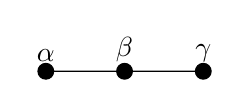
\begin{tikzpicture}
\draw[fill=black] 
(0,0) circle [radius=.1] node [above] {$\alpha$} --
(1,0) circle [radius=.1] node [above] {$\beta$} --
(2,0) circle [radius=.1] node [above] {$\gamma$};
\end{tikzpicture}.
  
For $m\geq 2$ define $G_m$ as the group presented by generators $\mathcal{X}_m$ and the following three families of relations:
\begin{align}
 \label{eq:am} \tag{$a_m$} x_{\alpha}(\xi) x_{\alpha}(\eta) & = x_{\alpha}(\xi+\eta),&  \xi,\eta\in B_d,\ d\leq m;&\\
 \label{eq:bm} \tag{$b_m$} [x_\alpha(\xi), x_{\alpha'}(\eta))] &  = 1, & \text{in the case $\alpha+\alpha'\not\in\Phi\cup\{0\}$,}\\
 \nonumber                                                     &       & \xi \in B_d,\ \eta \in B_e,\ d,e\leq m;\\
 \label{eq:cm} \tag{$c_m$} [x_\alpha(\xi), x_{\alpha'}(\eta)] & = x_{\alpha+\alpha'}(N_{\alpha,\alpha'}\xi\eta), & \text{in the case $\alpha+\alpha'\in \Phi$,}\\
 \nonumber                                                    &  & \xi \in B_d,\ \eta \in B_e,\ d, e, d+e \leq m.
 \end{align}
For $m=1$ define $G_1$ as the group presented by generators $\mathcal{X}_1$, 
three above families of relations $(a_1), (b_1), (c_1)$ and the following additional family:
\begin{align}  \label{eq:d1} \tag{$d_1$} [[x_{\alpha+\beta+\gamma}(\xi), x_{-\gamma}(\eta)], x_{\beta+\gamma}(\zeta) ] & = 1, 
 & \xi,\eta,\zeta\in B_1,\ \text{ $(\alpha, \beta, \gamma)$ is an $\rA_3$-triple. }
\end{align}

The obvious embedding of generators $\mathcal{X}_m \subseteq \mathcal{X}_{m+1}$ induces a map $f_m\colon G_m \to G_{m+1}$.
Our goal is to show the following result.
\begin{prop}\label{prop:tul3.3}
 For $m\geq 1$ the map $f_m$ is an isomorphism. Consequently, $\St(\Phi, B)$ can be presented by generators $\mathcal{X}_1$ and relations $(a_1)$, $(b_1)$, $(c_1)$, $(d_1)$.
\end{prop}
\begin{rem}
   Notice that for $\Phi=\rA_\ell$, $\ell\geq 4$ the group $\St(\Phi, B)$ admits a shorter presentation with family~ $(d_1)$ omitted (see~\cite[Lemma~3.3]{Tu83}).
   This is also true for $\Phi=\rE_\ell$ since $\St(\rE_\ell, R)$ can be presented as an amalgamated product of several copies of $\St(\rA_4, R)$, (cf. e.\,g.~\cite[Lemmas~3,7)]{S15}).   
  On the other hand, we believe that the above presentation is the shortest possible in the cases $\Phi=\rA_3, \rD_\ell$. \end{rem}

We will use the following commutator identities (cf.~\cite[H1]{Re75}):
\begin{align}
 \label{eq:H1ii}  [ab, c] = {}^a[b, c] \cdot [a,c];&\\ %= [a,[b,c]]\cdot [b,c] \cdot [a,c];&\\
 \label{eq:H1iii} [a,c]   = 1    \text{ implies } [a, [b,c]] = [[a,b],{}^bc].&
\end{align}

\begin{lemma}
 Suppose $m \geq 1$.
 Let $\alpha, \beta, \alpha', \beta' \in \Phi$ be such that $\alpha + \beta = \alpha' + \beta'$.
 Assume, moreover, that $\xi \in B_d$, $\xi' \in B_{d'}$, $\eta \in B_e$, $\eta' \in B_{e'}$ are such that 
  $N_{\alpha, \beta} \xi \eta = N_{\alpha', \beta'}\xi' \eta'$ for some $d,d',e,e'\leq m$ satisfying $d+e=d'+e' = m+1$.
 Then the following relations holds in $G_m$:
 \begin{equation}
  \label{eq:S-correctness} [x_\alpha(\xi), x_\beta(\eta)] = [x_{\alpha'}(\xi'), x_{\beta'}(\eta')].
 \end{equation}
 Moreover for every $\zeta \in B_{k''}$, $k''\leq m$ and $\gamma\in\{\alpha, \beta, \alpha + \beta\}$
  the following relation holds in $G_m$:
 \begin{equation}
 \label{eq:S-commutes} [[x_\gamma(\zeta), [x_\alpha(\xi), x_\beta(\eta)]] = 1.
 \end{equation}
\end{lemma}
\begin{proof}
 Notice that $k+l = m+1$, $k, l\leq m$ imply $k,l>0$, hence $B_i= A \cdot t^i$ for $i=k,k',l,'l'$.
 This means that without loss of generality we may assume that $\mathfrak{m}=0$ and $B = A[t]$.
 But now our statement is not different from~\cite[Proposition 1.1]{Re75} (or~\cite[Proposition~3.2.2]{RS76} in the case $g=1$)
  and can be proved by the same argument which remains valid for a general coeffient ring $A$.
\end{proof}

For every $\xi \in B_{m+1}$ and $\alpha\in \Phi$ there exist $\xi' \in B_m$ and $\alpha'\in \Phi$ such that $\xi = t\xi'$ and $\alpha-\alpha'\in\Phi$,
so we can define the following element of $G_m$:
\begin{equation} \label{eq:S-definition} S_\alpha(\xi) := [x_{\alpha-\alpha'}(N_{\alpha-\alpha',\alpha'} \xi'), x_{\alpha'}(t)].\end{equation} 
From~\eqref{eq:S-correctness} it follows that $S_\alpha(\xi)$ does not depend of the choice of $\alpha'$.

Let us show that elements $S_\alpha(\xi)$ satisfy the relations $(a_{m+1})$, $(b_{m+1})$ and $(c_{m+1})$.
From \eqref{eq:H1ii} and~\eqref{eq:S-commutes} it follows that $S_\alpha(\xi)$ satisfy $(a_{m+1})$ and hence $(b_{m+1})$ in the special case $\alpha=\alpha'$.
\begin{lemma} \label{lem:cm-plus1} Suppose that $m\geq 1$. For every $\alpha, \alpha' \in \Phi$ such that $\alpha+\alpha' \in \Phi$ and
 $a\in A$, $\xi \in B_d$, $d \leq 0$ the following relation holds in $G_m$: 
\begin{equation} \nonumber
[x_\alpha(\xi), S_{\alpha'}(at^{m+1})] = [x_\alpha(t\xi), x_{\alpha'}(at^m)] = S_{\alpha+\alpha'}(N_{\alpha,\alpha'}a\xi t^{m+1}).
\end{equation}
\end{lemma}
\begin{proof}
By \cite[Lemma~3.1.2]{RS76} we may assume without loss of generality that $\alpha'=\beta$ for some $\rA_3$-triple $(\alpha, \beta, \gamma)$.
\begin{align*}
   [x_\alpha(\xi), S_\beta(at^{m+1})] = [x_\alpha(\xi), [x_{\beta + \gamma}(t), x_{-\gamma}(a't^m)]]
   &  \text{ by~\eqref{eq:S-correctness},\eqref{eq:S-definition} for $a' = N_{\beta+\gamma, -\gamma} a$} \\ 
 = [x_{\alpha+\beta+\gamma}(\epsilon t\xi), {}^{x_{\beta+\gamma}(t)}x_{-\gamma}(a't^m)]             
 &  \text{ by~\eqref{eq:H1iii}, for $\epsilon=N_{\alpha, \beta+\gamma}$} \\
 = {}^{x_{\beta+\gamma}(t)}[x_{\alpha+\beta+\gamma}(\epsilon t\xi), x_{-\gamma}(a't^m)]             
 &  \text{ by $(b_1)$}
\end{align*} 
Denote by $R$ the expression in the right hand side of the above formula.
\begin{enumerate}
 \item \label{case:cm-1} Case $m=1$, $d = 0$.
 \begin{align*}
   R  = [x_{\alpha +\beta + \gamma}(\epsilon t\xi), x_{-\gamma}(a't)] 
   & \text{ by $(d_1)$}\\
      = {}^{x_{\beta+\gamma}(1)}[x_{\alpha +\beta + \gamma}(\epsilon t\xi), x_{-\gamma}(a't)] 
   & \text{ by~\eqref{eq:H1ii}, $(b_1)$, $(c_1)$} \\
      = [x_\alpha(\xi), [x_{\beta + \gamma}(1), x_{-\gamma}(a't^m)]] 
   & \text{ by $(b_1)$, \eqref{eq:H1iii}}\\
      = [x_\alpha(t\xi), x_\beta(at)]
   & \text{ by~\eqref{eq:S-correctness},\eqref{eq:S-definition}.}
 \end{align*}  
 \item \label{case:cm-2} Case $m\geq 2$ or $m=1$, $d < 0$.
 \begin{align*}
 R = {}^{x_{\beta+\gamma}(t)}[x_{\alpha+\beta+\gamma}(\epsilon t^2\xi), x_{-\gamma}(a't^{m-1})]     
 &  \text{ by~\eqref{eq:S-correctness} if $k=0$ or~\eqref{eq:cm} if $k <0$} \\
 = [[x_\alpha(t\xi), x_{\beta+\gamma}(t)], {}^{x_{\beta+\gamma}(t)} x_{-\gamma}(a't^{m-1})]         
 &  \text{ by~$(b_2)$, $(c_2)$ or by~\eqref{eq:S-commutes},\eqref{eq:S-definition} if $m=1$} \\
 = [x_\alpha(t\xi), x_\beta(at^m)]                                                                  
 &  \text{ by~\eqref{eq:H1iii}. \qedhere}
\end{align*} 

\end{enumerate}
\end{proof}

It will be convenient for us to extend the definition of $S_\alpha(\xi)$ by allowing $\xi$ to take values in $B_d$ for $d\leq m$.
In this case we simply set $S_\alpha(\xi) = x_\alpha(\xi)$.

Now suppose  $0 \leq d \leq m+1$. Clearly \eqref{eq:S-correctness} and \eqref{eq:S-definition} (in the case $1\leq d\leq m$) or~\cref{lem:cm-plus1} (in the case $d=0,m+1$) imply that
\begin{equation} \label{eq:cm-plus1-generalized} 
[S_\alpha(\xi), S_{\alpha'}(\eta)] = S_{\alpha+\alpha'}(N_{\alpha,\alpha'}\xi \eta),\ \xi \in B_d, \eta \in B_{m+1-d}.
\end{equation}

We need to introduce additional notation.
For $a,b\leq m+1$ we denote by $\bot(a, b)$ (resp. $\angle(a,b)$) the family of all relations $[S_\alpha(\xi), S_{\alpha'}(\eta)] = 1$
for which $\xi \in B_a$, $\eta \in B_b$ and $\alpha$ and $\alpha'$ are orthogonal (resp. form a sharp angle). 
We denote by $\bot_0(a, b)$ the subset of $\bot(a, b)$
consisting of those relations for which $\xi = t^{a} \in B_a$.

\begin{lemma} \label{claim1} In $G_m$ relations $\bot_0(1, d)$ and $\angle(d, m)$ imply $\angle(d, m+1)$ for $d\leq m+1$ \end{lemma}
\begin{proof}
Without loss of generality we may assume that $\alpha' = \alpha + \beta$
  for some $\rA_3$-triple $(\alpha, \beta, \gamma)$.
Write $\eta = bt^{m+1}$ for some $b\in A$.
\begin{align*} 
[S_\alpha(\xi), S_{\alpha+\beta}(bt^{m+1})] = [S_\alpha(\xi), [x_{\alpha+\beta+\gamma}(b't^m), x_{-\gamma}(t)]] & \text{ by~\eqref{eq:S-correctness} and~\eqref{eq:S-definition}}\\
= [[S_\alpha(\xi), x_{\alpha+\beta+\gamma}(b't^m)], {}^{x_{\alpha+\beta+\gamma}(b't^m)}\!x_{-\gamma}(t)] & \text{ by~$\bot_0(1, d)$}\\
= 1
 & \text{ by~$\angle(d, m)$. \qedhere} \end{align*} 
\end{proof}

\begin{lemma} \label{claim2} In $G_m$ relations $\angle(d, m+1)$ imply $\bot_0(d, m+1)$ for  $1\leq d\leq m+1$. \end{lemma}
\begin{proof}
As before, without loss of generality we may assume $\alpha' = \gamma$ for some $\mathsf{A}_3$-triple $(\alpha, \beta, \gamma)$.
 \begin{align*}
 {}^{S_\gamma(t^d)}S_\alpha(bt^{m+1}) = {}^{S_\gamma(t^d)}[S_{-\beta}(b't^{m+1}), x_{\alpha+\beta}(1)] & \text{ by~\cref{lem:cm-plus1}}\\
 = [S_{-\beta}(b't^{m+1}), {}^{S_\gamma(t^d)}x_{\alpha+\beta}(1)]                                     
 & \text{ by $\angle(d, m+1)$}\\
 = [[x_{-\beta-\gamma}(b''t^{m+1-d}), S_\gamma(t^d)], {}^{S_\gamma(t^d)}x_{\alpha+\beta}(1)]          
 & \text{ by~\eqref{eq:cm-plus1-generalized}}\\
 = [x_{-\beta-\gamma}(b''t^{m+1-d)}), [S_\gamma(t^d), x_{\alpha+\beta}(1)]]                           
 & \text{ by~\eqref{eq:H1iii} and $(b_{m+1-d})$}\\
 = S_{\alpha}(b'''t^{m+1})                                                                            
 & \text{ by~\eqref{eq:cm-plus1-generalized}.} \end{align*}
Usual identities for structure constants imply (cf.~\cite[p.~12]{Re75}):
 $b'''=N_{-\beta-\gamma, \alpha+\beta+\gamma} \cdot N_{\gamma, \alpha+\beta} \cdot N_{-\beta-\gamma, \gamma} \cdot N_{-\beta, \alpha+\beta} \cdot b = b,$ from which the claim follows.
\end{proof}

\begin{lemma} \label{claim3}
 In $G_m$ relations $\bot_0(d, m+1)$, $\angle(d, d)$ and $\angle(m+1, m+1)$ imply $\bot(d, m+1)$ for $d\leq m+1$.
\end{lemma}
\begin{proof}
 \begin{align*} 
 S_{\alpha+\beta+\gamma}(abt^{m+1}) = {}^{S_{-\beta}(t^d)}\!S_{\alpha+\beta+\gamma}(abt^{m+1}) 
 & \text{ by $\bot_0(d, m+1)$}\\
 = {}^{S_{-\beta}(t^d)}\![x_{\alpha+\beta}(b't^{m+1-d}), S_\gamma(at^d)] 
 & \text{ by~\eqref{eq:cm-plus1-generalized}} \\
 = [S_{\alpha}(b't^{m+1}) x_{\alpha+\beta}(b't^{m+1-d}), S_\gamma(at^d)] 
 & \text{ by~\eqref{eq:cm-plus1-generalized} and $\angle(d, d)$ }\\
 = {}^{S_{\alpha}(b't^{m+1})}\!S_{\alpha+\beta+\gamma}(abt^{m+1}) [S_{\alpha}(b't^{m+1}), S_\gamma(at^d)] 
 & \text{ by~\eqref{eq:H1ii} and~\eqref{eq:cm-plus1-generalized}} \\
 = S_{\alpha+\beta+\gamma}(abt^{m+1}) [S_{\alpha}(b't^{m+1}), S_\gamma(at^d)] 
 & \text{ by $\angle(m+1, m+1)$. \qedhere}
\end{align*}
\end{proof}

\begin{lemma} \label{lem:bm-plus1}
Elements $S_\alpha(\xi)$ satisfy relations $(b_{m+1})$.
 \end{lemma}
\begin{proof}
We must show that $S_\alpha(\xi)$ satisfy $\angle(d, m+1)$ and $\bot(d, m+1)$ for $d\leq m+1$.
\begin{enumerate}
 \item Relations $\angle(d, m+1)$, $d\leq m$ follow from~\cref{claim1}. 
 \item Relations $\bot(d, m+1)$ with $d\leq 0$ can verified by direct computation:
 \begin{align*} 
 [x_\alpha(\xi), S_{\gamma}(bt^{m+1})] = [x_\alpha(\xi), [x_{\beta+\gamma}(b't^m), x_{-\beta}(t)]] & \text{ by~\eqref{eq:S-correctness},\eqref{eq:S-definition}} \\
 = [[x_\alpha(\xi), x_{\beta+\gamma}(b't^m)], {}^{x_{\beta+\gamma}(b't^m)}\!x_{-\beta}(t)] &
 \text{ by \eqref{eq:H1iii} and $(b_1)$} \\
 = {}^{x_{\beta+\gamma}(b't^m)}\![x_{\alpha+\beta+\gamma}(b't^m\xi), x_{-\beta}(t)] &
 \text{ by $(b_m)$ and $(c_m)$} \\
 = 1 & \text{ by $(b_m)$.}
\end{align*}
 \item Relations $\bot_0(d, m+1)$ with $1\leq d\leq m$ follow from~\cref{claim2}.
 \item Relations $\angle(m+1, m+1)$ follow from~\cref{claim1}, consequently relations $\bot_0(m+1, m+1)$ follow from~\cref{claim2}.
 \item Relations $\bot(d, m+1)$, $0\leq d\leq m+1$ follow from~\cref{claim3} and the previous two assertions.
\end{enumerate}
\end{proof}

\begin{proof}[Proof of~\cref{prop:tul3.3}]
Define the map $g_m\colon G_{m+1} \to G_m$ by $g_m(x_\alpha(\xi)) = S_\alpha(\xi)$.
In view of the above lemmata this map is well-defined. It is clear that $g_m$ is inverse to $f_m$, which proves the first claim.

Denote by $G_\infty$ the group presented by generators $\mathcal{X}_\infty$ and relations $(a_\infty)$, $(b_\infty)$, $(c_\infty)$.
By the above argument there is an isomorphism between $G_1$ and $\colim\limits_{n\to\infty} G_n \cong G_\infty$.

Denote by $i\colon G_\infty \to \St(\Phi, B)$ the map induced by the obvious embedding of $\mathcal{X}_\infty$ into the set of 
 Steinberg generators of $\St(\Phi, B)$.  
Using~\eqref{eq:H1ii} multiple times it is not hard to show that the map $j\colon \St(\Phi, B) \to G_\infty$ given by
 $j(x_\alpha(b)) = \prod x_\alpha(b_i)$, where $b = \sum b_k$ is the decomposition of $b$ into a finite sum of its homogeneous components $b_k\in B_k$, is a well-defined map.
It is clear that $i$ and $j$ are mutually inverse. 
\end{proof}

\end{comment}

\section{Second injectivity theorem}
\begin{comment} 
First of all, set $\widetilde{V} = \overline{G}^{\geq 0}_M \times G^{\leq 0} \times (1 + M)^*$
 and consider it as a pointed set, i.\,e. ignore its structure of the group but retain $\widetilde{v_0} = (1, 1, 1)$ as a choice of a basepoint.
We let the group $\St(\Phi, R, M)$ act on $\widetilde{V}$ via the formula 
 $h \cdot (\overline{g}^+, g^-, u) = (\overline{g}^+ \cdot j_+i_+(h), i_-(h)^{-1}\cdot g^-, u)$.
Denote by $V$ the set of orbits of this action with the fixed basepoint $v_0 = O(\widetilde{v}_0)$.
We will use the notation $[\overline{g}^+, g^-, u]$ as a shorthand for $O(\overline{g}^+, g^-, u)$.

It is obvious that the map $\widetilde{p} \colon \widetilde{V} \to \St(\Phi, R[t, t^{-1}])$ given by 
 \[(\overline{g}^+, g^-, u) \mapsto \overline{g}^+ \cdot j_-(g^-) \cdot \{t, u\}\]
 is constant on the orbits of the above action
  and therefore gives rise to a well-defined map $p \colon V \to \St(\Phi, R[t, t^{-1}])$ of pointed sets.

We will construct an action of $\St(\Phi, B)$ on the set $V$ with the following additional properties:
\begin{enumerate}
\item for $g^- \in \St(\Phi, R[t^{-1}])$ one has $\varphi(g^-) \cdot v_0 = [1, g^-, 1]$, where $\varphi$ is the canonical map
  $\St(\Phi, R[t^{-1}]) \to \St(\Phi, B)$ induced by the embedding $R[t^{-1}] \to B$.
\item for $g \in \St(\Phi, B)$ the element $p(g \cdot v_0)$ coincides with the canonical image of $g$ in $\St(\Phi, R[t, t^{-1}])$; 
\end{enumerate} \end{comment}

\subsection{Lemma33}
Throughout this section $\Phi$ is a simply-laced irreducible root system and $A$ is a local ring with maximal ideal $M$.

For a simply-laced root system $\Phi$ and a commutative ring $R$, the Steinberg group $\St(\Phi,\,R)$ is generated by the formal symbols $x_{\alpha}(a)$ for $\alpha\in\Phi$, $a\in R$ subject to the Steinberg relations
\begin{align}
&x_{\alpha}(a)x_{\alpha}(b)=x_{\alpha}(a+b), \tag{R1}\\
&[x_{\alpha}(a),\,x_{\beta}(b)]=x_{\alpha+\beta}(N_{\alpha\beta}\,ab),\text{ for }\alpha+\beta\in\Phi, \tag{R2} \\
&[x_{\alpha}(a),\,x_{\beta}(b)]=1,\text{ for }\alpha+\beta\not\in\Phi\cup0. \tag{R3}
\end{align}

Let $I\trianglelefteq A$ be a (not neccesarily proper) ideal of a commutative ring $A$. Denote $R=\oplus_{d\in\mathbb Z}R_d\subseteq A[t,t\inv]$, where $R_d=It^d$, $d<0$, and $R_d=At^d$, $d\geq0$.

For such a ring $R$ one can assume in the definition of the Steinberg group that the generators $x_\alpha(a)$ and relations R1--R3 are defined only for homogeneous elements. 

Consider the root system $\rD_l$ for $l\geq5$. It can be naturally embedded into the root system of type $\rC_l$ as a set of short roots.

Define truncated Steinberg groups $G_n$ for $n\geq1$ by the set of generators $x_\alpha(a)$, $\alpha\in\rD_l$, $a\in R_d$, $d\leq n$, and relations

\begin{align}
&\,\,x_{\alpha}(a)x_{\alpha}(b) =  x_{\alpha}(a+b),& a,b\in R_d,\ d\leq n, \tag{R$1_n$} \\
&\,[x_{\alpha}(a),\,x_{\beta}(b)]= x_{\alpha+\beta}(N_{\alpha\beta}\,ab),& a\in R_d,\ b\in R_e,\ d,e,d+e\leq n, \tag{R$2_n$} \\
&[x_{\alpha}(a),\,x_{\beta}(b)]= 1,& \alpha+\beta\not\in\rC_l\cup0,\ a\in R_d,\ b\in R_e,\ d,e\leq n, \tag{R$3.1_n$} \\
&[x_{\alpha}(a),\,x_{\beta}(b)]= 1,& \alpha+\beta\in\rC_l\setminus\rD_l,\ a\in R_d,\ b\in R_e,\ d,e,d+e\leq n. \tag{R$3.2_n$}
\end{align}

\begin{rem}
We can take $\mathbb R^l$ with a base $\chi_1,\ldots,\chi_l$ and visualise root systems
\[\rD_l=\{\pm\chi_i\pm\chi_j\mid1\leq i\neq j\leq l\}\]
and $\rC_l=\rD_l\cup\{\pm2\chi_i\mid1\leq i\leq l\}$. Then we immediately see that $\alpha+\beta\in\rC_l\setminus\rD_l$ exactly means that either $\{\alpha,\beta\}$ or $\{-\alpha,-\beta\}$ equals $\{\chi_i-\chi_j,\chi_i+\chi_j\}$. Then for some $\sigma$ from the Weyl group of $\rD_l$ we get 
\[ \{\sigma\alpha,\sigma\beta\}=\{\chi_{l-1}-\chi_l, \chi_{l-1}+\chi_l\}=\{\alpha_{l-1},\alpha_l\} \]
(the horns of the Dynkin diagram $\rD_l$). Another condition on $\alpha$ and $\beta$ equivalent to $\alpha+\beta\in\rC_l\setminus\rD_l$ is that they do not lie in any subsystem of $\rD_l$ of type $\rA_m$ for $m\geq4$.
\end{rem}

We claim that $G_n\cong G_{n+1}$, more precisely, we construct an inverse homomorhism to the natural map $G_n\rightarrow G_{n+1}$. With this end we define elements $s_\alpha(a)\in G_n$ for $a\in R_{n+1}$ and prove the above relations for these elements. We start with the following easy fact.

\begin{lemma}
\label{welldef}
Take $d$, $e\leq n$, $d+e=n+1$, $a\in R_d$, $b\in R_e$, and consider an embedding $\iota\colon\rA_4\hookrightarrow\rD_l$. For the chosen simple roots $\alpha_k$ of $\rA_4$ denote $\beta_k=\iota(\alpha_k)$. Then holds
\[ [x_{\beta_1}(a),\,x_{\beta_2+\beta_3}(b)]=[x_{\beta_1+\beta_2}(Nabt\inv),\,x_{\beta_3}(t)], \]
where $N=N_{\beta_1,\beta_2}N_{\beta_2,\beta_3}$.
\end{lemma}
\begin{proof}
Observe that $d$, $e\geq1$. Take $x=x_{\beta_1}(a)$, $y=x_{\beta_2}(N_{\beta_3,\beta_2}bt\inv)$, $z=x_{\beta_3}(t)$. Since $x$ and $z$ lie in the subsystem of type $\rA_4$, we get by R3.1$\!\,_n$ that they commute. Then Hall--Witt identity gives us
\[ \,^y[x,\,[y\inv,\,z]]=\,^x[[x\inv,\,y],\,z], \]
where $[x,\,[y\inv,z]]=[x_{\beta_1}(a),\,x_{\beta_2+\beta_3}(b)]$ and $[[x\inv,y],\,z]=[x_{\beta_1+\beta_2}(Nabt\inv),\,x_{\beta_3}(t)]$ by R2$\!\,_n$. Here $x$ commutes with $x_{\beta_1+\beta_2}(Nabt\inv)$ and $x_{\beta_3}(t)$, and $y$ commutes with $x_{\beta_2+\beta_3}(b)$ by R3.1$\!\,_n$. Finally, $[x_{\beta_1}(-a),\,y]=x_{\beta_1+\beta_2}(Nabt\inv)$ also commutes with $x_{\beta_2+\beta_3}(b)$, what finishes the proof.
\end{proof}

The above lemma allows us for $a\in R_{n+1}$ and $\alpha\in\rD_l$ chose an arbitrary decomposition $\alpha=\beta+\gamma$ and define $s_\alpha(a)=[x_\beta(N_{\beta,\gamma}\,at\inv),\,x_\gamma(t)]$. Indeed, take another decomposition $\alpha=\beta'+\gamma'$, we may assume that subsystem $\Psi$ generated by $\beta$, $\beta'$, $\gamma$, $\gamma'$ has type $\rA_3$ If it is contained in the subsystem of type $\rA_4$, we are done by Lemma~\ref{welldef}. If not, we may assume $\Psi=\langle\alpha_{l-2},\alpha_{l-1},\alpha_l\rangle$ and since $l\geq5$ take two subsystems of type $\rA_4$, say, $\Psi_1$ and $\Psi_2$, which overlap by $\rA_3$, and $\beta$, $\gamma\in\Psi_1$, $\beta'$, $\gamma'\in\Psi_2$. Therefore, there exist $\beta''$, $\gamma''\in\Psi_1\cap\Psi_2$ with $\alpha=\beta''+\gamma''$ and we can again apply Lemma~\ref{welldef} to get the claim. 

Moreover, with the assumption of Lemma~\ref{welldef} on $a$ and $b$ we have
\[ [x_{\beta}(a),\,x_{\gamma}(b)]=s_{\alpha}(N_{\beta,\gamma}\,ab). \]

The following observation is obvious.
\begin{lemma} \label{commute}
Consider an embedding $\iota\colon\rA_4\hookrightarrow\rD_l$ and denote $\beta_k=\iota(\alpha_k)$ for simple roots $\alpha_k$ of $\rA_4$. Then for any $a\in R_d$, $b\in R_e$, $c\in R_f$ with $d$, $e$, $f\leq n$ holds
\[ [[x_{\beta_1}(a),\,x_{\beta_2}(b)],\,x_{\beta_4}(c)]=1. \]
\end{lemma}

Consider now any two roots $\alpha$, $\beta\in\rD_l$ such that $\alpha+\beta\not\in\rC_l\cup0$. Since $l\geq5$, there exists a subsystem $\Psi$ of type $\rA_4$, containing $\alpha$ and $\beta$. Then we can take any $a\in R_{n+1}$ and $b\in R_d$ for $d\leq n$ and apply Lemma~\ref{commute} for $\Psi$ to get
\begin{equation} \label{sx} [s_\alpha(a),\,x_\beta(b)]=1. \end{equation}
Next, using this fact we can apply again Lemma~\ref{commute} for $\Psi$ and get
\[ [s_\alpha(a),\,s_\beta(c)]=1 \]
for any $c\in R_{n+1}$. Therefore, R3.1$\!\,_{n+1}$ holds for $s_\alpha$'s.

Now one can take $a\in R_d$ for $d\leq0$ and $b\in R_{n+1}$, and repeat the proof of Lemma~\ref{welldef} using~(\ref{sx}) to get
\[ [x_\beta(a),\,s_\gamma(b)]=\begin{cases}s_{\beta+\gamma}(N_{\beta\gamma}\,ab),&d=0,\\x_{\beta+\gamma}(N_{\beta\gamma}\,ab),&d<0.\end{cases} \]
This finishes the proof of R2$\!\,_{n+1}$.

The proof of R1$\!\,_{n+1}$ is left to the reader. The next lemma is devoted to R3.2$\!\,_{n+1}$.

\begin{lemma} For $a\in R_d$, $b\in R_e$, $d$, $e\leq n$, $d+e=n+1$ holds \[ [x_{\alpha_{l-1}}(a),\,x_{\alpha_l}(b)]=1. \] \end{lemma}
\begin{proof} Take $x=x_{\alpha_{l}-\alpha_{l-2}}(N_{\alpha_{l}-\alpha_{l-2},\alpha_{l-2}}bt\inv)$, $y=x_{\alpha_{l-1}-\alpha_{l-2}}(N_{\alpha_{l-2},\alpha_{l-1}-\alpha_{l-2}}at\inv)$, and $z=x_{\alpha_{l-2}}(t)$. Then
\[ [x_{\alpha_{l-1}}(a),\,x_{\alpha_l}(b)]=[[y\inv,\,z],\,[x,\,z]]=\,^{y\inv z}[y,\,[z\inv,\,x]]\cdot[y\inv,\,[x,\,z]]. \]
Next, by R3.2$\!\,_n$ we know that $x$ and $y$ commute, and therefore 
\[ \,^{y\inv z}[y,\,[z\inv,\,x]]=[[y\inv,\,z],\,x]=x_{\alpha_{l-1}+\alpha_{l}-\alpha_{l-2}}(Nabt\inv) \]
for $N=N_{\alpha_{l-1},\alpha_{l}-\alpha_{l-2}}N_{\alpha_{l}-\alpha_{l-2},\alpha_{l-2}}$. Finally,
\[ [y\inv,\,[x,\,z]]=x_{\alpha_{l-1}-\alpha_{l-2}+\alpha_l}(N'abt\inv) \]
for $N'=-N_{\alpha_{l-2},\alpha_{l-1}-\alpha_{l-2}}N_{{\alpha_{l-1}-\alpha_{l-2}},\alpha_l}$. Since $N_{\alpha,\beta}$ are the structure constants of the Lie algebra, it follows $N=-N'$ from the Jacobi identity.
\end{proof}

Now the same argument as in Lemma~\ref{welldef} allows to prove that $[s_{\alpha_{l-1}}(a),\,x_{\alpha_l}(b)]=1$ for $b\in R_e$, $e\leq0$, what finishes the proof of R3.2$\!\,_{n+1}$.

\subsection{Computation of the kernel of the map of evaluation at \texorpdfstring{$0$}{0}.}
For a pair $(R, I)$ we denote by $\overline{\St}(\Phi, R, I)$ the image of the map $\mu$ from~\eqref{relSteinberg-def}, in particular, it is a normal subgroup of $\St(\Phi, R)$.
We also denote by $\St(\Phi, I)$ the subgroup of $\St(\Phi, R)$ generated as a group by root unipotents of level $I$.
It is clear that $\overline{\St}(\Phi, R, I)$ contains $\St(\Phi, I)$ and, in fact, is its normal closure.
We also denote by $\overline{H}(\Phi, R, I)$ the subgroup of $\overline{\St}(\Phi, R, I)$ generated by the semisimple root elements $h_\alpha(u)$ and symbols $\{u, v\}$, $u \in (1+I)^*$, $v \in R^*$, $\alpha\in \Phi$.

The aim of this subsection is to describe the kernel of the map $ev_{X=0}^*\colon\overline{\St}(\Phi, A[X], M[X]) \to \overline{\St}(\Phi, A, M)$
induced by the ring homomorphism of evaluation at $0$. Clearly, this kernel, denote it by $K(A[X], M[X])$, contains the subgroup $\overline{\St}(\Phi, A[X], XM[X])$, however, apriori it may be larger, so our goal will be to describe the explicit extra elements sufficient to generate it.

Obviously, $ev_{X=0}^*$ admits a section hence we can consider $\overline{\St}(\Phi, A, M)$ and $\St(\Phi, M)$ as subgroups of $\overline{\St}(\Phi, A[X], M[X])$,
 moreover, the following decomposition holds:
\begin{equation} \label{relZero-decomp} \overline{\St}(\Phi, A[X], M[X]) = \overline{\St}(\Phi, A, M) \cdot K(A[X], M[X]).\end{equation}
\begin{lemma} The following decomposition holds
 \[ K(A[X], M[X]) = \overline{\St}(\Phi, A[X], XM[X]) \cdot \left[\St(\Phi, XA[X]),\ \overline{\St}(\Phi, A, M)\right].\] \end{lemma}
\begin{proof} Fix $g \in K(A[X], M[X])$ and write it as $g(X) = \prod_i z_{\alpha_i}(f_i(X), \xi_i(X))$ for some $f_i(X) = f_i(0) + Xf_i'(X) \in M[X]$, $\xi_i(X) = \xi_i(0) + X\xi_i'(X) \in A[X]$.
 It is clear that modulo $\overline{\St}(\Phi, A[X], XM[X])$ the element $g(X)$ is congruent to $g_1(X) = \prod_i z_{\alpha_i}(f_i(0), \xi_i(X)).$ 
 
 Now each factor $z_{\alpha_i}(f_i(0), \xi_i(X))$ can be written as follows:
 \[z_{\alpha_i}(f_i(0), \xi_i(0))^{x_{-\alpha_i}(X\xi'_i(X))} = [x_{-\alpha_i}(-X\xi'_i(X)), z_{\alpha_i}(f_i(0), \xi_i(0))] \cdot z_{\alpha_i}(f_i(0), \xi_i(0)).\]
 Since the subgroup $C = \left[\St(\Phi, XA[X]), \overline{\St}(\Phi, A, M)\right]$ is normalized by $\overline{\St}(\Phi, A, M)$ 
 (this follows e.\,g. from the formula $[g, h]^{h_1} = [h_1^{-1}, g][g, h_1^{-1}h]$) we conclude that $g_1(X)$ is congruent to $\prod_i z_{\alpha_i}(f_i(0), \xi_i(0)) = g(0) = 1$ modulo $C$,
 which implies the assertion. \qedhere \end{proof}

\begin{theorem}[Stein] \label{thmStein} For a local ring $A$ with maximal ideal $M$ holds \[\overline{\St}(\Phi, A, M) = U(\Phi^+, M) \cdot \overline{H}(\Phi, A, M) \cdot U(\Phi^-, M).\] \end{theorem} \begin{proof} See~\cite[Theorem~2.4]{Ste73}. \end{proof}

\begin{prop} \label{Kgen} For $A$ and $M$ as above the subgroup $K(A[X], M[X])$ is generated as a group by its subgroup $\overline{\St}(\Phi, A[X], XM[X])$ and
 the elements $[x_\alpha(m), x_{-\alpha}(X\xi)]$, $m \in M$, $\xi \in A[X]$, $\alpha \in \Phi$. \end{prop}
\begin{proof} Notice that it follows from~\eqref{eq:conj-h-x} $\overline{H}(\Phi, A, M)$ normalizes both $\St(\Phi, XA[X])$ and $\St(\Phi, M)$ and, moreover, that $[\overline{H}(\Phi, A, M),\ \St(\Phi, XA[X])] \subseteq \overline{\St}(\Phi, A[X], XM[X])$. 
 
Now for $g \in \St(\Phi, XA[X])$, $h \in \overline{H}(\Phi, A, M)$, $u^+ \in U(\Phi^+, M)$, $u^- \in U(\Phi^-, M)$ holds:
\[ [g, h u^+ u^-] = [g, h] \cdot [{}^{h}\!g, {}^{h}\!(u^+u^-)] \in \St(\Phi, A[X], XM[X]) \cdot [\St(\Phi, XA[X]), \St(\Phi, M)],\]
hence $\left[\St(\Phi, XA[X]), \overline{\St}(\Phi, A, M)\right] \subseteq \overline{\St}(\Phi, A[X], XM[X]) \cdot \left[\St(\Phi, XA[X]), \St(\Phi, M)\right]$ and therefore \[K(A[X], M[X]) = \overline{\St}(\Phi, A[X], XM[X]) \cdot \left[\St(\Phi, XA[X]),\ \St(\Phi, M)\right].\]
 
It is clear that modulo $\overline{\St}(\Phi, A[X], XM[X])$ the commutator subgroup $[\St(\Phi, XA[X]), \St(\Phi, M)]$ is generated by elements of the form $[x_\alpha(m), x_{-\alpha}(X\xi)]^g$, where $m \in M$, $\xi \in A[X]$, $g \in \St(\Phi, A[X])$.
Thus, to verify the assertion it remains to show that the commutators $[[x_\alpha(m), x_{-\alpha}(X\xi)], g]$ belong to $\overline{\St}(\Phi, A[X], XM[X])$.
Since the latter subgroup is normal it suffices to prove this inclusion in the special case when $g$ is a member of some generating set for $\St(\Phi, A[X])$.
Clearly, the set consisting of $x_\beta(\xi)$, $\xi \in A[X]$, $\beta \neq \pm \alpha$ is such a generating set, but in this case the required inclusions follow from~\eqref{C1}--\eqref{C3} of~\cref{Crels}. \end{proof}

\begin{corollary} \label{Kgen-strong} For $A$ and $M$ as in~\cref{thmStein} and arbitrary fixed root $\gamma$ of an irreducible simply-laced root system $\Phi$ the subgroup $K(A[X], M[X])$ is generated as a group by $\overline{\St}(\Phi, A[X], XM[X])$ and the elements $c_{\gamma}(m, X\eta)$, where $m \in M$, $\eta \in A[X]$. \end{corollary}
\begin{proof} Substituting $\xi = 1$, $s = m$, $t = X\eta$ into relation~\eqref{C4} of~\cref{Crels} we obtain that modulo 
 $\overline{\St}(\Phi, A[X], XM[X])$ the element $c_{\alpha + \beta}(m, X\eta)$ is equivalent to $c_{\alpha}(-\epsilon m, -\epsilon X \eta)^{-1}$, $\epsilon = N_{\alpha, \beta}$. The assertion of the corollary now easily follows from the irreducibility of $\Phi$.
\end{proof}

\subsection{The subgroups \texorpdfstring{$P_\alpha(0)$}{Pa(0)}, \texorpdfstring{$P_\alpha(*)$}{Pa(*)} and their properties.} 
For a root system $\Phi$ consider the following subsets of $\Phi$:
\begin{align} Z_+(\alpha) & = \{ \beta \in \Phi \mid \langle \alpha, \beta \rangle > 0 \}, \\
   Z_0(\alpha) & = \{ \beta \in \Phi \mid \alpha + \beta \not\in \Phi,\ \langle \alpha, \beta \rangle = 0 \}, \\
   Z(\alpha)   & = Z_0(\alpha) \sqcup Z_+(\alpha). \end{align} 
Clearly, $Z_0(\alpha)$ (resp. $Z_+(\alpha)$) is a reductive (resp. special) subset of $\Phi$.
   
We denote by $Z_\alpha(A, M)$ the subgroup of $\overline{\St}(\Phi, A, M)$ generated by elements
 $x_{\beta}(m),\ \beta \in Z_+(\alpha)$ and $z_{\gamma}(m, \zeta),\ \gamma \in Z_0(\alpha),$ where $m \in M$, $\zeta \in A$.
It is not hard to see that \[Z_\alpha(A, M) = \Img\left(\overline{\St}(Z_0(\alpha), A, M) \to \overline{\St}(\Phi, A, M)\right) \rtimes \hat{U}(Z_+(\alpha), M). \]
It is clear, that $Z_\alpha(A, M)$ centralizes the root subgroup $X_\alpha(A)$ (cf. \cite[984]{St71}).

For the rest of this subsection $\Phi$ is a simply-laced root system of rank $\geq 3$ and $\alpha$ is a root of $\Phi$. Notice that in the simply-laced case the assumption $\alpha+\beta\not\in \Phi$ in the definition of $Z_0(\alpha)$ is superfluous, i.\,e. $Z_0(\alpha) = \{ \alpha\in\Phi \mid \alpha \perp \beta \}$
(cf.~\cite[Proposition~5.7]{St71}).

\begin{rem}\label{Z-DS} Notice that our assumptions on the rank of $\Phi$ guarantee that $Z_0(\alpha)$ is nonempty, hence the group $Z_\alpha(A, M)$ contains relative Dennis--Stein symbols $\langle a, m \rangle$ for $a\in A$, $m\in M$.
By~\eqref{DS-S-relationship} relative Steinberg symbols $\{a, 1+m\}$ are also contained in $Z_\alpha(A, M)$ for all $a\in A^*$, $m\in M$. \end{rem}

\begin{df} \label{defP0} Denote by $P_\alpha(0)$ the subgroup of $\St(\Phi, A[X, X^{-1}])$ generated by the images of the following elements of $\St(\Phi, A[X])$ under the
 map $j_+ \colon \overline{\St}(\Phi, A[X], M[X]) \to \St(\Phi, A[X, X^{-1}])$:
\begin{enumerate} \item $z_{\beta}(Xf, \xi), \beta \in \Phi \text{ such that }\alpha + \beta \in \Phi\text{ or } \alpha - \beta \in \Phi;$
 \item $z_{\beta}(f, X\xi),\ \alpha - \beta \in \Phi;$
 \item $z_{\beta}(f, \xi),\ \beta \perp \alpha;$
 \item $x_{-\alpha}(X^2f);$
 \item $x_{\alpha}(f)$. \end{enumerate}
In the above formulae and for the rest of this subsection $f \in M[X]$ and $\xi \in A[X]$. \end{df}

\begin{rem}\label{rem:c-DS} It is easy to check that $P_\alpha(0)$ contains the image of $Z_\alpha(A, M)$ under the natural embedding of $\St(\Phi, A, M) \hookrightarrow \St(\Phi, A[X, X\inv])$.
In particular, it contains the relative Dennis--Stein and Steinberg symbols.
It is also clear that $P_\alpha(0)$ contains the elements $c_{\beta}(f, X\xi)$ for all $\beta \in Z(\alpha)$
 (they can be factored as products of two elements of type 2 or 3). \end{rem}

Denote by $P_\alpha(*)$ the subgroup of $\St(\Phi, A[X, X^{-1}])$ generated by $P_\alpha(0)$ and the elements $x_{-\alpha}(mX)$, $m \in M$.
The following lemma shows that the resulting subgroup is sufficiently large.
\begin{lemma} \label{Pstar-large} The subgroup $P_\alpha(*)$ contains the image of $K(A[X], M[X])$ in $\St(\Phi, A[X, X^{-1}])$. \end{lemma}
\begin{proof} Clearly, $P_\alpha(*)$ contains the elements $x_\beta(Xf)$ for all $\beta \in \Phi$ and $z_\beta(Xf, \xi)$ for $\beta \in \Phi \setminus \{\pm \alpha\}$, $f \in M[X]$, $\xi\in A[X]$ hence by~\cref{thm:Stepanov} $P_\alpha(*)$ contains whole $j_+(\overline{\St}(\Phi, A[X], XM[X]))$. The required assertion now follows from~\cref{Kgen-strong} and the preceding remark. \end{proof}

\begin{rem} \label{Pstar-char} The above lemma allows us to characterize $P_\alpha(*)$ as follows: it consists precisely of images under $j_+$ of all elements 
 $g \in \overline{\St}(\Phi, A[X], M[X])$ for which $ev_{X=0}^*(g)$ lies in the subgroup $Z_\alpha(A, M)$. \end{rem} 
   
\begin{lemma}\label{P0_normal} The subgroup $P_\alpha(0)$ is normal in $P_\alpha(*)$. In particular, there is an exact sequence, which is split by the map $m \mapsto x_{-\alpha}(mX)$:
\[\xymatrix{1 \ar[r] & P_\alpha(0) \ar[r] & P_\alpha(*) \ar[r]^{p_\alpha} & M^+ \ar@<5pt>@{-->}[l] \ar[r] & 1}.\] \end{lemma}
\begin{proof} We need to verify that the conjugate by $x_{-\alpha}(mX)$ to every generator $g$ of $P_\alpha(0)$ listed in~Definition~\ref{defP0} belongs to $P_\alpha(0)$.
The assertion is obvious for the generators of type 3 and 4.

Suppose $g$ has type 1 or 2 and $\alpha - \beta \in \Phi$. By~\cref{Zrels} we obtain that
\begin{align} z_{\beta}(Xf, \xi) ^ {x_{-\alpha}(mX)} = & x_{-\alpha} (- mX^2f\xi) \cdot x_{\beta-\alpha} (N_{\beta, -\alpha}\cdot mX^2f) \cdot z_{\beta}(Xf, \xi), \label{eq3-1} \\
  z_{\beta}(f, X\xi) ^ {x_{-\alpha}(mX)} = & x_{-\alpha} (- mX^2f\xi ) \cdot x_{\beta-\alpha} (N_{\beta, -\alpha}\cdot mXf) \cdot z_{\beta}(f, X\xi), \label{eq3-2} \end{align}
The expressions in the right hand sides of~\eqref{eq3-1} and~\eqref{eq3-2} are products of generators of type 4, 1, 1 and 4, 1, 2, respectively.  

Suppose $g$ has type 1 and  $\alpha + \beta \in \Phi$. By~\cref{Zrels} 
\begin{equation} \label{eq3-3} z_{\beta}(Xf, \xi) ^ {x_{-\alpha}(mX)} = x_{-\alpha} (mX^2f\xi ) \cdot x_{-\alpha-\beta} (N_{\beta,\alpha}\cdot mX^2f\xi^2) \cdot z_{\beta}(Xf, \xi). \end{equation}
and the latter expression is a product of generators of type $4, 1, 1$.

Finally, suppose $g$ has type $5$.
Substituting in~\eqref{Z5} of~\cref{Zrels} $s = -\epsilon f$, $\xi = -\epsilon m$, $\eta=X$ and expressing $z_\alpha(f, mX)$ through other terms we obtain that
\begin{multline} \label{eq:zalpha} z_\alpha(f, mX) = x_{\alpha+\beta}(\epsilon Xf) \cdot x_{\beta}(-mX^2 f) \cdot x_{-\beta}(mf) \cdot x_\alpha(f) \cdot \\ 
 \cdot z_{\alpha+\beta}(-\epsilon X f, -\epsilon m) \cdot z_{-\beta}(-mf, -X) \cdot x_{-\alpha-\beta}(-\epsilon m^2X f) \cdot x_{-\alpha}(-m^2X^2 f), \end{multline}
and the latter expression is a product of generators of type 1, 1, 2, 5, 1, 2, 1, 4. \end{proof}

\begin{rem} \label{rem:palpha} From the two preceding lemmas it follows that the value of the function $p_\alpha$ from the statement of~\cref{P0_normal} on an element $g\in K(A[X], M[X])$ can be computed via the following procedure. 
Start with any presentation of $g$ as a product of elements $z_{\beta}(Xf, \xi)$ for $\beta \in \Phi$ and $c_\delta(f, X\xi)$ for some fixed $\delta\in Z_0(\alpha)$. 
Now pick among these factors those that correspond to the root $\beta = -\alpha$ (i.\,e. pick all factors $z_{-\alpha}(Xf_i, \xi_i)$). 
Now $p_\alpha(g)$ is precisely the sum of constant terms of the polynomials $f_i$. \end{rem}

For $m \in M$ denote by $P_\alpha(m)$ the coset $P_\alpha(0) \cdot x_{-\alpha}(mX)$.
From the preceding lemma it follows that $P_\alpha(*)$ coincides with the union of all $P_\alpha(m)$, $m\in M$. This allows us to make the following definition. 

\begin{df} Define the map $S_\alpha(a, -) \colon P_\alpha(*) \to \St(\Phi, A[X, X^{-1}])$ on each coset $P_\alpha(m)$, $m \in M$ via the following formula:
\[ S_\alpha(a, g) = x_\alpha(aX^{-1})\cdot g \cdot x_\alpha\left(-\tfrac{aX^{-1}}{1 + am}\right) \cdot \{X, 1+ am\}_\alpha.\] \end{df}
It follows immediately from the definition of $S_\alpha(a, -)$ that for $g_1 \in P_\alpha(m)$, $g_2 \in P_\alpha(*)$ holds
\begin{equation} \label{eq:Smult} S_\alpha(a, g_1\cdot g_2) = S_\alpha(a, g_1) \cdot S_\alpha\left(\tfrac{a}{1+am}, g_2\right).\end{equation}

It is clear that the restriction of the map $S_\alpha(a, g)$ to the subgroup $P_\alpha(0)$ coincides with the map of left conjugation by $x_\alpha(aX^{-1})$.

\begin{lemma}\label{P0_conj} The subgroup $P_\alpha(0)$ is stable under conjugation by $x_\alpha(aX^{-1})$ for arbitrary $a\in A$. \end{lemma}
\begin{proof} We need to verify that the conjugate by $x_\alpha(aX^{-1})$ to every generator $g = z_\beta(f, \xi)$ from~\cref{defP0} lies in $P_\alpha(0)$. 
The assertion is clear for generators of type 3 and 5.
First of all, consider the case $\alpha + \beta \in \Phi$, which is only possible for the generator of type 1:
\begin{equation}\label{eq:Zconj1} z_{\beta}(Xf, \xi) ^ {x_{\alpha}(aX^{-1})} = x_{\alpha} (- afg) \cdot x_{\alpha+\beta} (N_{\beta, \alpha}\cdot af) \cdot z_{\beta}(Xf, \xi). \end{equation}
Clearly, the expression in the right hand side is a product of generators of type 5, 2, 1. 

Now consider the case $\alpha - \beta \in \Phi$, which is possible for the generators of type 1 and 2.
Computing the conjugates of these generators using~\cref{Zrels} we obtain that
\begin{align} z_{\beta}(Xf, \xi) ^ {x_{\alpha}(aX^{-1})} = &  x_{\alpha} (af\xi) \cdot x_{\alpha-\beta} (N_{\beta,-\alpha}\cdot af\xi^2) \cdot z_{\beta}(Xf, \xi), \label{eq:Zconj2} \\
z_{\beta}(f, X\xi) ^ {x_{\alpha}(aX^{-1})} = & x_{\alpha} (af\xi) \cdot x_{\alpha-\beta} (N_{\beta,-\alpha}\cdot aXf\xi^2) \cdot z_{\beta}(f, X\xi). \nonumber \end{align}
The expressions in the right-hand side are products of generators of type 5, 2, 1 and 5, 1, 2.

Let us verify the assertion for the generator of type 4.
Choose $\beta\in \Phi$ such that $\alpha+\beta \in \Phi$. 
Substituting $s = Xf$, $\eta = X$, $\xi = aX^{-1}$ and $\alpha = -\alpha - \beta$ into~\eqref{Z5} of~\cref{Zrels} we obtain that
\begin{multline} \label{eq:Zconj3} z_{-\alpha}(X^2f, aX^{-1}) = x_{-\alpha-\beta}(\epsilon Xf) \cdot x_{-\beta}(-af) \cdot x_{\beta}(aX^2 f) \cdot x_{-\alpha}(X^2f) \cdot \\
 \cdot z_{-\alpha-\beta}(-\epsilon Xf, -\epsilon a) \cdot x_{\alpha+\beta}(-\epsilon a^2 Xf) \cdot x_{\alpha}(- a^2 f) \cdot z_{-\beta}(a f, -X), \end{multline}
where $\epsilon = N_{-\alpha-\beta,\beta}$. 
Clearly, the expression in the right-hand side is a product of generators of type 1, 2, 1, 4, 1, 1, 5, 2. \end{proof}

\begin{lemma} \label{lem:Tulenbayev-formula} 
One has $S_\alpha(a, x_{-\alpha}(mX)) = x_{-\alpha}\left(\tfrac{mX}{1+am}\right) \cdot \langle a, m\rangle_\alpha \cdot h_\alpha(1+am).$
\end{lemma}
\begin{proof} Since $\Phi$ is nonsymplectic, we can choose $\gamma \in \Phi$ such that $\langle \alpha, \gamma \rangle = -1$. Direct computation using~\eqref{eq:conj-h-x},\eqref{eq:conj-h-h},\eqref{eq:steinberg},\eqref{eq:dennis-stein} shows that
 \begin{multline*}
 x_\alpha(aX^{-1}) \cdot x_{-\alpha}(mX) = {}^{h_\gamma(X)}(x_\alpha(a) \cdot x_{-\alpha}(m)) = \\
 = {}^{h_\gamma(X)}\left( x_{-\alpha}\left(\tfrac{m}{1+am}\right) \cdot \langle a, m\rangle_\alpha \cdot h_\alpha(1+am) \cdot x_\alpha\left(\tfrac{a}{1+am}\right) \right) = \\
 = x_{-\alpha}\left(\tfrac{mX}{1+am}\right) \cdot \langle a, m\rangle_\alpha \cdot h_\alpha(X^{-1}(1+am))\cdot h_\alpha(X^{-1})^{-1} \cdot x_{\alpha}\left(\tfrac{aX^{-1}}{1+am}\right) = \\
 = x_{-\alpha}\left(\tfrac{mX}{1+am}\right) \cdot \langle a, m\rangle_\alpha \cdot \{1+am, X^{-1}\}^{-1} \cdot h_\alpha(1+am)\cdot x_{\alpha}\left(\tfrac{aX^{-1}}{1+am}\right) = \\
 = x_{-\alpha}\left(\tfrac{mX}{1+am}\right) \cdot \langle a, m\rangle_\alpha \cdot h_\alpha(1+am) \cdot x_{\alpha}\left(\tfrac{aX^{-1}}{1+am}\right) \cdot \{1+am, X\}, \end{multline*}
which implies the assertion. \end{proof}

\begin{corollary} For $g \in P_\alpha(m)$ holds $S_\alpha(a, g) \cdot h_\alpha^{-1}(1 + am) \in P(\alpha, \tfrac{m}{1 + am})$.
Consequently one has \[ S_\alpha(a+b, g) = S_\alpha\left(b,\ S_\alpha(a, g) \cdot h_\alpha^{-1}(1 + am)\right)\cdot h_\alpha(1+am). \]\end{corollary} \begin{proof}
Fix an element $g \in P_\alpha(m)$ and write it $g = g_0 \cdot x_{-\alpha}(mX)$ for some $g_0 \in P_\alpha(0)$.
Now by~\eqref{eq:Smult} and~\cref{P0_conj} one has
\begin{multline} \nonumber S_\alpha(a, g) \cdot h_{\alpha}^{-1}(1+am) = S_\alpha(a, g_0) \cdot S_\alpha(a, x_{-\alpha}(mX)) \cdot h_{\alpha}^{-1}(1+am) = 
\\ = S_\alpha(a, g_0) \cdot x_{-\alpha}\left(\tfrac{mX}{1+am}\right) \cdot\langle a, m \rangle \in P_\alpha\left(\tfrac{m}{1+am}\right). \end{multline}

The second assertion can be verified directly using~\eqref{eq:symbol-properties}. \end{proof}

\subsection{The subgroups \texorpdfstring{$K(\alpha, \beta)$}{K(a,b)} and their properties}
Throughout this subsection $\alpha, \beta$ denote a fixed pair of roots of $\Phi$ forming a sharp angle (i.\,e. $\langle \alpha, \beta \rangle = 1$). We denote by $\Psi$ the subsystem of type $\rA_2$ generated by $\alpha$ and $\beta$.
\begin{df} Denote by $K(\alpha, \beta)$ the subgroup of $\St(\Phi, A[X, X^{-1}])$ generated by the following elements:
 \begin{enumerate}
  \item $z_\gamma(Xf, \xi)$, for all $\gamma \in \Phi \setminus \Psi$;
  \item $x_{-\alpha}(X^2f)$, $x_{-\beta}(X^2f)$;
  \item $x_{\alpha}(Xf)$, $x_\beta(Xf)$;
  \item $x_{\alpha-\beta}(Xf)$, $x_{\beta-\alpha}(Xf)$;
  \item $c_{\delta}(f, X\xi)$ for some fixed root $\delta \in \Phi \setminus \Psi$. \end{enumerate} \end{df}

\begin{prop} \label{K-a-b} Every element $g \in K(A[X], M[X])$ can be written as a product $g_0 \cdot x_{-\alpha}(mX) \cdot x_{-\beta}(m'X)$ for some $m, m' \in M$ and $g_0 \in K(\alpha, \beta)$. Consequently, $K(\alpha, \beta)$ coincides with the intersection $K(A[X], M[X]) \cap P_\alpha(0) \cap P_\beta(0)$. \end{prop}
\begin{proof} Denote by $\Sigma$ the special part of the parabolic subset $S = \Psi \cup \Phi^+$. Applying~\cref{thm:Stepanov} to $S$ we obtain that every element of $\St(\Phi, A[X], XM[X])$ can be presented as a product of $z_\gamma(Xf, \xi)$, $\gamma \in \Sigma(S) \subseteq \Phi\setminus \Psi$ and $x_\gamma(Xf)$, $\gamma \in \Psi$. By~\cref{Kgen-strong} we can write $g$ as a product of these generators and generators of type 5.
  
 The next step of the proof is to decompose each factor of the form $x_{\epsilon}(Xf)$, $\epsilon \in \{-\alpha,-\beta\}$ appearing in this product as
 $x_{\epsilon}(X^2f') \cdot x_{\epsilon}(mX)$ and then move $x_{\epsilon}(mX)$ to the rightmost position conjugating by $x_{\epsilon}(mX)$ all factors along the way.
 Notice that no terms of the form $x_{\epsilon}(mX)$, $\epsilon \in \{ -\alpha, -\beta \}$ may appear after simplification of these conjugates, so this process is guaranteed to terminate.
 To see this notice that the extra terms in the right-hand sides of \eqref{eq3-1} and~\eqref{eq3-3} 
 (as well as all terms in the right-hand sides of~\eqref{C1},\eqref{C2} of~\cref{Crels} if one substitutes corresponding values into them) have terms of degree at least $2$ in $X$. 
  
 As a side effect of this transformation, however, factors $x_\alpha(Xf)$ and $x_\beta(Xf)$ appearing in $g$ might transform into factors of the form $z_\alpha(Xf, X\xi)$, and $z_\beta(Xf, X\xi)$. We can express each factor $z_\alpha(Xf, X\xi)$ through the generators of $K(\alpha, \beta)$ as follows. Pick a root $\gamma \in \Phi\setminus \Psi$ forming an obtuse angle with $\alpha$ and then invoke~\eqref{eq:zalpha}:
 \begin{multline} z_\alpha(Xf, X\xi) = x_{\alpha+\gamma}(\epsilon X^2f) \cdot x_{\gamma}(-X^3 \xi f) \cdot x_{-\gamma}(Xf\xi) \cdot x_\alpha(Xf) \cdot \\ 
 \cdot z_{\alpha+\gamma}(-\epsilon X^2 f, -\epsilon \xi) \cdot z_{-\gamma}(-Xf\xi, -X) \cdot x_{-\alpha-\gamma}(-\epsilon X^2\xi^2 f) \cdot x_{-\alpha}(-X^3 f \xi^2),\ \text{for } \epsilon = N_{\alpha, \gamma}. \end{multline}
 The expression in the right-hand side is a product of generators of type 1, 1, 1, 3, 1, 1, 1, 2. Similar argument also applies to $z_\beta(Xf, X\xi)$.  
 
 After collecting terms $x_\epsilon(mX)$, $\epsilon \in \{ -\alpha, -\beta \}$ in the right-hand side of the resulting expression we obtain the desired decomposition for $g$.
 
 It is clear from the definition that $K(\alpha, \beta) \subseteq P_\alpha(0) \cap P_\beta(0) \cap K(A[X], M[X])$. The reverse inclusion follows from the just proved decomposition and the fact that for $g\in K(A[X], M[X])$ one has $p_{\alpha}(g) = m$ and $p_\beta(g) = m'$ (cf.~\cref{rem:palpha}). \end{proof}
 
 We need one more technical definition.
\begin{df} Denote by $Z_{\alpha, \beta}$ the subgroup of $\St(\Phi, A[X, X^{-1}])$ generated by elements $z_\gamma(f, X\xi)$, where $\gamma \in Z_+(\alpha) \setminus \{ \alpha - \beta \}$.\end{df}
  
\begin{lemma} \label{image-K-a-b} The image of $K(\alpha, \beta)$ under $S_{\alpha}(a, -)$ is contained in the subgroup of $\St(\Phi, A[X, X^{-1}])$  generated by $K(\alpha, \beta)$ and $Z_{\alpha, \beta}$. \end{lemma}
\begin{proof} To simplify notation we call the generators of the subgroup $Z_{\alpha,\beta}$ ``generators of type Z``. By~\eqref{eq:Zconj1}, \eqref{eq:Zconj2} the conjugate to each generator $z_\gamma(Xf, \xi)$ of type 1 by $x_\alpha(aX^{-1})$ is a product of generators of type Z, Z, 1.
By~\eqref{eq:Zconj3} the conjugate to the generator $x_{-\alpha}(X^2f)$ is a product of generators of type 1, Z, 1, 2, 1, 1, Z, Z.
The conjugation by $x_\alpha(aX^{-1})$ fixes both generators of type 3 and transforms $x_{-\beta}(X^2f)$ into a product of generators of type 2, 1. As for the remaining generators of type 5, \cref{Crels} shows that the corresponding conjugate can be written as a product of generators of type Z, Z, 5. \end{proof}  

\begin{corollary} The image of $K(\alpha, \beta)$ under $S_\alpha(a, -)$ is contained in $P_\beta(0)$. \end{corollary}
\begin{proof} Follows from the above lemma and the fact that the generators of $Z_{\alpha,\beta}$ are generators of type 2 for $P_\beta(0)$ in the sense of~\cref{defP0}.
 Indeed, if $\gamma \in Z_+(\alpha) \setminus \{ \alpha - \beta \}$ is such that $\langle \beta, \gamma \rangle = -1$, then $ \langle \alpha - \beta, \gamma \rangle \geq 2$, hence
  $\gamma = \alpha - \beta$, a contradiction. \end{proof}

\begin{lemma} \label{lem:SRsharp} For $g \in K(A[X], M[X]) \cap P_\alpha(m) \cap P_\beta(m')$ and $a \in A$ holds \[S_\alpha(a, g)\cdot  h^{-1}_\alpha(1 + am) \cdot x_{\alpha-\beta}(-N_{\alpha,-\beta}\cdot m'a) \in P_\beta\left(\tfrac{m'}{1 + am}\right). \] \end{lemma}
\begin{proof} By~\cref{K-a-b} $g$ can be presented as $ g_0 \cdot x_{-\alpha}(mX) \cdot x_{-\beta}(m'X)$ for some $g_0\in K(\alpha, \beta)$, therefore from~\eqref{eq:Smult} and~\cref{lem:Tulenbayev-formula} we obtain that \begin{multline} \nonumber S_\alpha(a, g) = S_\alpha(a, g_0) \cdot S(a, x_{-\alpha}(mX)) \cdot S_\alpha\left(\tfrac{a}{1+am}, x_{-\beta}(m'X)\right) = \\ = S_\alpha(a, g_0) \cdot \langle a, m \rangle \cdot h_\alpha(1+am) \cdot x_{-\beta}(m'X) \cdot x_{\alpha-\beta}\left(\tfrac{N_{\alpha, -\beta} \cdot m'a}{1+am}\right) = \\ =
  S_\alpha(a, g_0) \cdot \langle a, m \rangle \cdot  x_{-\beta}\left(\tfrac{m'X}{1+am}\right) \cdot x_{\alpha-\beta}\left(N_{\alpha, -\beta} \cdot m'a\right) \cdot h_\alpha(1+am). \end{multline}
The assertion now follows from the preceding corollary.
\end{proof}
  
\begin{lemma} \label{conj-K-a-b} For $b \in A$ one has $K(\alpha, \beta)^{x_{\beta - \alpha}(b)} \subseteq K(\alpha, \beta)$. \end{lemma}
\begin{proof} By~\eqref{Z2}--\eqref{Z4} of~\cref{Zrels} the conjugate to the generator $g=z_\gamma(Xf, \xi)$ of type 1 by $x_{\beta-\alpha}(b)$ either coincides with $g$ or is a product of generators of type 4, 1, 1. Now if $g = x_\epsilon(Xf)$, $\epsilon \in \{\pm \alpha, \pm \beta\}$ is a generator of type 2 or 3, the conjugation by $x_{\beta-\alpha}(a)$ either fixes $g$ or transforms it into a product of two generators of type 2 or 3. By~\eqref{C1}--\eqref{C3} of~\cref{Crels} the conjugate to a generator $g = c_\delta(f, X\xi)$ of type 5 either coincides with $g$ or is a product of generators of type 5, 4, 1. Finally, from~\cref{rem:palpha} we obtain that $z_{\alpha-\beta}(Xf, b) \in K(A[X], M[X]) \cap P_\alpha(0) \cap P_{\beta}(0) = K(\alpha, \beta)$. \end{proof} 

\begin{lemma} For $g \in K(\alpha, \beta)$ and $a, b\in A$ the conjugate to $S_\alpha(a, g)$ by $x_{\beta-\alpha}(b)$ belongs to $P_\alpha(0)$. \end{lemma}
\begin{proof} By~\cref{image-K-a-b} and~\cref{conj-K-a-b} it remains to show that the conjugate to each generator $g = z_\gamma(f, X\xi)$, $\gamma \in Z_+(\alpha) \setminus \{ \alpha - \beta \}$ of $Z_{\alpha, \beta}$ by $x_{\beta-\alpha}(b)$ belongs to $P_\alpha(0)$. Throughout the proof we understand generator types according to~\cref{defP0}. It is clear that $g$ itself is a generator of type 2, therefore it remains to consider the case $\gamma\not \perp \beta - \alpha$. 
 
 In the case $\alpha - \beta - \gamma \in \Phi$ we obtain from \eqref{Z2} of~\cref{Zrels} that
\[ z_{\gamma}(f, X\xi) ^ {x_{\beta-\alpha}(b)} = x_{\beta-\alpha} (- bXf\xi) \cdot x_{-\alpha + \gamma + \beta} (N_{\gamma, \beta -\alpha}\cdot bf)     \cdot z_{\gamma}(f, X\xi)\ \text{if}\ \alpha - \beta - \gamma \in \Phi. \] Notice that $\langle \alpha - \beta - \gamma, \alpha \rangle = \langle \alpha, \alpha \rangle - \langle \beta, \alpha \rangle - \langle \gamma, \alpha \rangle \leq 2 - 1 - 1 = 0$, 
 hence $\langle \alpha - \beta - \gamma, \alpha \rangle = -1,0$ and the expression in the right-hand side is a product of generators of type 1, 2, 2 or 1, 3, 2.

Now suppose that the other alternative holds, namely that $\alpha - \beta + \gamma \in \Phi$.
Since $\langle \alpha - \beta + \gamma, \alpha \rangle = \langle \alpha , \alpha \rangle - \langle \beta, \alpha \rangle + \langle \gamma, \alpha \rangle \geq 2 - 1 + 1 = 2$
we obtain that $\alpha - \beta + \gamma = \alpha$. Thus, by \eqref{Z3} of~\cref{Zrels}
\[z_{\gamma}(f, X\xi) ^ {x_{\beta-\alpha}(b)} = x_{\beta-\alpha} (bXf\xi) \cdot x_{-\alpha} (N_{\gamma,\alpha - \beta}\cdot bX^2 f\xi^2) \cdot z_{\gamma}(f, X\xi). \]
The expression in the right-hand side is a product of generators of type 1, 4, 2. \end{proof}

\begin{lemma} \label{lem:SRobtuse} For $g \in K(A[X], M[X]) \cap P_\alpha(m) \cap P_\beta(m')$ and $a, b\in A$ the element \[ x_{\beta - \alpha}(b) \cdot S_\alpha(a, g) \cdot h_{\alpha}^{-1}(1+am)\cdot h_{\beta - \alpha}((1 + \epsilon abm')^{-1})\cdot x_{\beta - \alpha}(-b(1 + \epsilon abm')) \]
 belongs to $P_\alpha\left(\tfrac{m - \epsilon bm'}{1+am}\right)$, where $\epsilon = N_{\alpha, -\beta}$.
\end{lemma}
\begin{proof} Set $c = 1 + \epsilon a b m'$, $s_0 = \langle a, m \rangle$, $s_1 = \langle \epsilon am', -bc^{-1} \rangle$.
From the definition of $S_\alpha(a, -)$ we obtain that
 \begin{multline} \label{eq:SRobtuse-computation}
 S_\alpha(a, x_{-\beta}(m'X) \cdot x_{-\alpha}(mX)) \cdot h_{\alpha}^{-1}(1+am)\cdot h_{\beta-\alpha}(c^{-1})\cdot x_{\beta - \alpha}(-bc) = \\ 
 = S_\alpha(a, x_{-\beta}(m'X)) \cdot S_\alpha(a, x_{-\alpha}(mX)) \cdot h_\alpha^{-1} (1 + am) \cdot h_{\beta - \alpha}(c^{-1}) \cdot x_{\beta - \alpha}(-bc) = \\
 = x_{-\beta}(m'X) \cdot x_{\alpha - \beta}(\epsilon am') \cdot x_{\beta - \alpha}(-bc^{-1}) \cdot x_{-\alpha}\left(\tfrac{mX}{1+am}\right) \cdot s_0 \cdot h_{\beta - \alpha}(c^{-1}) = \\
 = x_{-\beta}(m'X) \cdot x_{\beta - \alpha}(-b) \cdot s_1 \cdot h_{\alpha-\beta}(c^{-1}) \cdot x_{\alpha-\beta}\left(\epsilon acm'\right) \cdot x_{-\alpha}\left(\tfrac{mX}{1+am}\right) \cdot s_0 \cdot h_{\beta - \alpha}(c^{-1}) = \\
 =  x_{\beta - \alpha}(-b) \cdot x_{-\beta}(m'X) \cdot x_{-\alpha}(-\epsilon bm'X) \cdot s_1 \cdot x_{\alpha-\beta}(\epsilon ac^{-1}m') \cdot x_{-\alpha}\left(\tfrac{cmX}{1+am}\right) \cdot s_0 = \\
 = x_{\beta-\alpha}(-b) \cdot x_{-\beta}\left(m'X(1 - \epsilon abm'c^{-1})\right) \cdot x_{\alpha-\beta}(\epsilon ac^{-1}m') \cdot s_1 \cdot s_0 \cdot x_{-\alpha}\left(-\epsilon bm' X + \tfrac{cmX}{1+am}\right).
\end{multline}
Denote by $h_0$ the product of all terms except the first and the last one in the above formula. It is clear that $h_0$ lies in $P_\alpha(0)$. Using~\cref{K-a-b} we can decompose $g = g_0 \cdot x_{-\beta}(m'X) \cdot x_{-\alpha}(mX)$ for some $g_0 \in K(\alpha, \beta)$. The required assertion now follows from \eqref{eq:Smult}, \eqref{eq:SRobtuse-computation} and the preceding lemma:
\begin{multline} \nonumber
 x_{\beta - \alpha}(b) \cdot S_\alpha(a, g) \cdot h_{\alpha}^{-1}(1+am)\cdot h_{\beta - \alpha}(c^{-1})\cdot x_{\beta - \alpha}(-bc) = \\
  = x_{\beta - \alpha}(b) \cdot S_\alpha(a, g_0) \cdot x_{\beta-\alpha}(-b) \cdot h_0 \cdot x_{-\alpha}\left(\tfrac{m -\epsilon bm'}{1+am}\right) \in P_\alpha(\tfrac{m -\epsilon bm'}{1+am}). \qedhere
\end{multline}
\end{proof}

\subsection{The proof of the injectivity theorem}
We denote by $B$ the ring $M[X] + A[X^{-1}]$ considered as a graded subring of $A[X, X^{-1}]$.
For shortness we also write $G_M^0$ instead of $\overline{\St}(\Phi, A, M)$.
\[ \xymatrix{ G_M^0 \ar@{^{(}->}[r]^{i_+} \ar@{^{(}->}[d]^{i_-} & \overline{\St}(\Phi, A[X], M[X]) \ar^{j_+^M}[d] \ar@{^{(}->}[r] & \St(\Phi, A[X]) \ar[dl]^{j_+} \\
              \St(\Phi, A[X\inv]) \ar[r]^{j_-} & \St(\Phi, A[X, X^{-1}]) &  } \] 
Denote by $\overline{G}^{\geq 0}_M$ the image of the map $j_+^M$. 
Denote by $V$ the subset of $\St(\Phi, A[X, X^{-1}]) \times \St(\Phi, A[X\inv]) \times (1 + M)^*$ consisting of those triples $(g, h, u)$ for which 
$p(g, h, u) := g \cdot j_-(h) \cdot \{ X, u \}$ belongs to $\overline{G}_M^{\geq 0}$.
We let $h_0 \in G_M^0$ act on $V$ on the right by $(g, h, u) \cdot h_0 = (g, h \cdot i_-(h_0), u)$.
It is clear that this action is well defined.
Denote by $\overline{V}$ the set of orbits of the action of $G_M^0$ on $V$.
Whenever $(g, h_1, u)$ and $(g, h_2, u)$ lie in the same orbit we use the notation $(g, h_1, u) \sim (g, h_2, u)$.

The next step of the proof is to define for $\alpha \in \Phi$, $a \in A$ a partial function $t_\alpha(aX^{-1}) \colon V \not\to V$.
This function is defined for those triples $(g, h, u)$ for which $p(g, h, u) \in P_\alpha(*) \subseteq \overline{G}_M^{\geq 0}$.
If $p(g, h, u) \in P_\alpha(m)$ for some $m \in M$, then $t_\alpha(aX^{-1})$ is given by the following identity:
\[ t_\alpha(aX^{-1}) (g, h, u) = \left( x_\alpha(aX^{-1})\cdot g ,\ h \cdot x_\alpha\left(-\tfrac{aX^{-1}}{1 + am}\right),\ u \cdot (1 + am)\right).\]
It is easy to verify that $p(t_\alpha(aX^{-1}) (g, h, u)) = S_\alpha(a, p(g, h, u)).$

\begin{lemma} Let $\Phi$ be a simply-laced root system of rank $\geq 3$, $(A, M)$ be a local pair. Then for $\alpha \in \Phi$ the partial function $t_\alpha(aX^{-1}) \colon V \not \to V$ descends to a well-defined total function 
  $T_\alpha(aX^{-1}) \colon \overline{V} \to \overline{V}$. \end{lemma}
\begin{proof}
 First of all, let us show that the resulting function is total. 
 Fix $(g, h, u) \in V$. Since $p(g, h, u) \in \overline{G}^{\geq 0}_M$ there exists $g_1 \in \overline{\St}(\Phi, A[X], M[X])$ such that $j_+(g_1) = p(g, h, u).$
 Set $h_0 = ev^*_{X=0}(g_1)^{-1}$, then, clearly, $g_1 \cdot i_+(h_0) \in K(A[X], M[X])$ and 
 $p(g, h \cdot i_-(h_0), u) = j_+(g_1) \cdot j_-(i_-(h_0)) = j_+(g_1 \cdot i_+(h_0)) \in j_+(K(A[X], M[X])) \subseteq P_\alpha(*)$,
  which shows that $t_\alpha(aX^{-1})$ is defined on $(g, h \cdot i_+(h_0), u)$, which is also a representative of the same orbit as $(g, h, u)$.
  
 Next, let us show that the value of $T_\alpha(aX^{-1})$ does not depend on the choice of a representative.
 Let $(g, h_1, u) \sim (g, h_2, u)$ be elements of the same orbit for which both $p(g, h_1, u)$ and $p(g, h_2, u)$ belong to $P_\alpha(*)$.
 By definition, $h_1^{-1} h_2 = i_-(h_0)$, for some $h_0 \in G^0_M$, moreover, 
  $p(g, h_1, u)^{-1} \cdot p(g, h_2, u) = j_- i_-(h_0) = j_+ i_+(h_0) \in P_\alpha(*)$.
 By~\cref{Pstar-char} there exists $g_1 \in \overline{\St}(\Phi, A[X], M[X])$ such that $g_0 := ev^*_{X=0}(g_1) \in Z_\alpha(A, M)$ and $j_+(g_1) = j_+ i_+ (h_0)$.
 From the last equality and the injectivity of the map $G(\Phi, A[X]) \to G(\Phi, A[X, X^{-1}])$ we obtain that
 the projections of $g_0$, $g_1$ and $h_0$ in $G(\Phi, A[X, X^{-1}])$ are equal, which shows that $g_0 \cdot h_0^{-1} \in \overline{\K_2}(\Phi, A, M)$. 
 By~\cref{thmStein} the latter subgroup is generated by relative Steinberg symbols $\{ a, 1 + m \}$ and therefore is contained in $Z_\alpha(A, M)$ by~\cref{Z-DS}. Thus, we have obtained that $h_0 \in Z_\alpha(A, M)$ and hence that $i_-(h_0)$ is centralized by $X_\alpha(A[X^{-1}])$, which allows us to conclude that
 \begin{multline} \nonumber
  t_\alpha(aX^{-1})(g, h_1, u) = \left( x_\alpha(aX^{-1})\cdot g ,\ h_1 \cdot x_\alpha\left(-\tfrac{aX^{-1}}{1 + am}\right),\ u \cdot (1 + am)\right) \sim \\
  \sim \left( x_\alpha(aX^{-1})\cdot g ,\ h_1 i_-(h_0) \cdot x_\alpha\left(-\tfrac{aX^{-1}}{1 + am}\right),\ u \cdot (1 + am)\right) = t_\alpha(aX^{-1})(g, h_2, u). \qedhere
 \end{multline} \end{proof}

\begin{comment}
The next step of the proof is to pass from the set $V_0'$ to its quotient $V_0$ 
We allow multiplying the second component on the right by an element of $\mathrm{im}(\St(\Phi, A, M) \to \St(\Phi, A))$
 (this operation is well defined for $V'_0$).

\begin{multline}
 T_\alpha(bX^{-1}) T_\alpha(aX^{-1}) \left(g,\ h,\ u\right) \sim \\ \sim
T_\alpha(bX^{-1}) \left(x_\alpha(aX^{-1})\cdot g,\ h \cdot x_\alpha\left(-\tfrac{aX^{-1}}{1 + am}\right) \cdot h^{-1}_\alpha(1 + am),\ u(1 + am)\right) = \\
 = \left( x_\alpha\left((a+b)X^{-1}\right)\cdot g,\ h',\ u(1 + am + bm) \right) \sim T_\alpha((a+b)X^{-1}) \left( g,\ h,\ u\right),\text{ since} \end{multline} 
 \begin{multline}
h' = h \cdot x_\alpha\left(-\tfrac{aX^{-1}}{1+am}\right) \cdot h^{-1}_\alpha(1+am) \cdot x_\alpha\left(-\tfrac{bX^{-1}}{1 + \tfrac{bm}{1+am}}\right) = \\ = 
 h \cdot x_\alpha\left(- \tfrac{aX^{-1}}{1 + am} - \tfrac{bX^{-1}}{(1+am)(1 + am + bm)}\right) \cdot h^{-1}_\alpha(1+am) \sim  
  h \cdot x_\alpha\left(- \tfrac{(a+b)X^{-1}}{1 + am + bm}\right).
\end{multline}

If $\alpha + \beta \not \in \Phi$ but $\alpha - \beta \in \Phi$, $\pi(g, h, u) \in P(\alpha, m) \cap P(\beta, m')$ then
$S_\alpha(a, \pi(g, h, u))\cdot  h^{-1}_\alpha(1 + am) \cdot x_{\alpha-\beta}(-N_{\alpha-\beta, \beta}m'a) \in P(\beta, \tfrac{m'}{1 + am})$
%($\beta = 2r$, $\alpha = 1r$, $\gamma = 12$, $\gamma = \alpha - \beta$)
\begin{multline}
 T_\beta(bX^{-1}) T_\alpha(aX^{-1}) \left(g, h, u\right) = 
 T_\beta(bX^{-1}) \left(x_\alpha(aX^{-1})\cdot g,\ h \cdot x_\alpha\left(-\tfrac{aX^{-1}}{1 + am}\right) ,\ u(1 + am)\right) \sim \\ 
 \sim T_\beta(bX^{-1}) \left(x_\alpha(aX^{-1})\cdot g,\ h \cdot x_\alpha\left(-\tfrac{aX^{-1}}{1 + am}\right) \cdot h^{-1}_\alpha(1 + am) \cdot x_{\alpha-\beta}(-m'a),\ u(1 + am)\right) = \\
 = (x_\beta(bX^{-1}) x_\alpha(aX^{-1}) \cdot g, h', u(1 + am + bm')), \text{ where} \end{multline} 
 \begin{multline}
 h' = h \cdot x_\alpha\left(-\tfrac{aX^{-1}}{1 + am}\right) \cdot h^{-1}_\alpha(1 + am) \cdot x_{\alpha-\beta}(-N_{\alpha-\beta, \beta}m'a) \cdot x_\beta\left(-\tfrac{bX^{-1}(1+am)}{1 + am + bm'}\right) \sim \\
    \sim h \cdot x_\alpha\left(-\tfrac{aX^{-1}}{1 + am}\right) \cdot h^{-1}_\alpha(1 + am) \cdot x_{\alpha}\left(\tfrac{m'abX^{-1}(1+am)}{1 + am + bm'}\right) \cdot x_\beta\left(-\tfrac{bX^{-1}(1+am)}{1 + am + bm'}\right) = \\
 = h \cdot x_\alpha\left(-\tfrac{aX^{-1}}{1 + am} + \tfrac{m'abX^{-1}}{(1+am)(1 + am + bm')}\right) \cdot x_\beta\left(-\tfrac{bX^{-1}(1+am)^{1 -\langle \beta, \alpha \rangle}}{1 + am + bm'}\right) \cdot h^{-1}_\alpha(1 + am) \sim \\
 \sim h \cdot x_\alpha\left(-\tfrac{aX^{-1}}{1 + am + bm'}\right) \cdot x_\beta\left(-\tfrac{bX^{-1}}{1 + am + bm'}\right).
\end{multline}
The latter expression is symmetric.

\begin{align*} {}^{x_\gamma(X^{-1})}x_\alpha(bX^{-1}) = {}^{x_\gamma(X^{-1})}[x_{-\beta}(b'X^{-1}), x_{\alpha+\beta}(1)] & \text{ by R$2_1$}\\
 = [x_{-\beta}(b'X^{-1}), {}^{x_\gamma(X^{-1})}x_{\alpha+\beta}(1)] & \text{ by R$3_1$ for sharp angles}\\
 = [[x_{-\beta-\gamma}(b''), x_\gamma(X^{-1})], {}^{x_\gamma(X^{-1})}x_{\alpha+\beta}(1)] & \text{ by R$2_1$}\\
 = [x_{-\beta-\gamma}(b''), [x_\gamma(X^{-1}), x_{\alpha+\beta}(1)]] & \text{ by R$3_0$}\\
 = x_{\alpha}(b'''X^{-1}) & \text{ by R$2_1$.} \end{align*}

\begin{align*} x_{\alpha+\beta+\gamma}(abX^{-1}) = {}^{x_{-\beta}(X^{-1})}\!x_{\alpha+\beta+\gamma}(abX^{-1}) & \text{ by the above relation}\\
 = {}^{x_{-\beta}(X^{-1})}\![x_{\alpha+\beta}(b'), x_\gamma(aX^{-1})] & \text{ by R$2_1$} \\
 = [x_{\alpha}(b'X^{-1}) x_{\alpha+\beta}(b'), x_\gamma(aX^{-1})] & \text{ by R$2_1$ and R$3_1$ for sharp angles }\\
 = {}^{x_{\alpha}(b'X^{-1})}\!x_{\alpha+\beta+\gamma}(abX^{-1}) [x_{\alpha}(b'X^{-1}), x_\gamma(aX^{-1})] & \text{ by R$2_1$} \\
 = x_{\alpha+\beta+\gamma}(abX^{-1}) [x_{\alpha}(b'X^{-1}), x_\gamma(aX^{-1})] & \text{ by R$3_1$ for sharp angles.} \end{align*}
\end{comment}
\printbibliography
\end{document}
